\documentclass[../main.tex]{subfiles}

\usepackage{nopageno} %Seitenzahlen auf richtiger Seite 

\usepackage[left=2cm, right=2cm, top=2cm, includehead, includefoot, headheight=17pt]{geometry}

\usepackage[utf8x]{inputenc}
\usepackage[english]{babel}
\usepackage{amsmath,amssymb,amsthm}
\usepackage{framed}
\usepackage{wasysym}
\usepackage[T1]{fontenc} %Silbentrennung 
\usepackage{color} %Farbe
\usepackage{graphicx}
\usepackage{float}%Grafik am gleichen Ort plazieren
%pdf. png. einfach eingliedern
\usepackage{subfigure} %Grafiken nebeneinander
\usepackage{pdfpages}
\usepackage{ulem} 	%\uuline{urgent}    % doppelt unterstreichen
%\uwave{boat}      % unterschlängeln
%\sout{wrong}       % durchstreichen
%\xout{removed}     % ausstreichen mit //////.

\usepackage{tikz}
\usetikzlibrary{trees}
\usetikzlibrary{plotmarks}
\usetikzlibrary{angles,quotes,babel}
\usetikzlibrary{shadings}
\usetikzlibrary{patterns}
\usetikzlibrary{matrix}
\usetikzlibrary{arrows}
\usetikzlibrary{calc}

\usepackage{pgfplots}
\usepackage{pgf-pie}
\pgfplotsset{compat=1.10}
\usepgfplotslibrary{statistics}
\usepgfplotslibrary{fillbetween}

\usepackage{tkz-euclide}
\usepackage{enumerate}
\usepackage{stmaryrd}
\usepackage{tabularx}
\usepackage{wrapfig}
\usepackage{epsdice}
\usepackage{multirow}
\usepackage{rotating}
\usepackage{pdflscape}
\usepackage{fancyhdr}

\pagestyle{fancy} %eigener Seitenstil
\fancyhf{} %alle Kopf- und Fußzeilenfelder bereinigen
\fancyhead[L]{} %Kopfzeile links
\fancyhead[C]{} %zentrierte Kopfzeile
\fancyhead[R]{} %Kopfzeile rechts
\renewcommand{\headrulewidth}{0.4pt} %obere Trennlinie
\fancyfoot[C]{\thepage} %Seitennummer
\renewcommand{\footrulewidth}{0.4pt} %untere Trennlinie

% Number spaces 
\newcommand{\CC}{\ensuremath{\mathbb{C}}}
\newcommand{\RR}{\ensuremath{\mathbb{R}}}
\newcommand{\QQ}{\ensuremath{\mathbb{Q}}}
\newcommand{\ZZ}{\ensuremath{\mathbb{Z}}}
\newcommand{\NN}{\ensuremath{\mathbb{N}}}
\newcommand{\LL}{\ensuremath{\mathbb{L}}}
\newcommand{\DD}{\ensuremath{\mathbb{D}}}
\newcommand{\WW}{\ensuremath{\mathbb{W}}}

%draw chemestry molecules 
\usepackage{chemfig} % https://mirror.ox.ac.uk/sites/ctan.org/macros/generic/chemfig/

\newcommand\vv[1]{%
	\begin{tikzpicture}[baseline=(arg.base)]
		\node[inner xsep=0pt] (arg) {$#1$};
		\draw[line cap=round,line width=0.45,->,shorten >= 0.2pt, shorten <= 0.7pt] (arg.north west) -- (arg.north east);
	\end{tikzpicture}%
} %command will render \vv{x} with an arrow aboth 

\renewcommand{\labelenumi}{\roman{enumi})}

\DeclareMathOperator{\ggT}{ggT}
\DeclareMathOperator{\sign}{sign}

%sections
\theoremstyle{plain}
\newtheorem{Thm}{Theorem}[section]
\newtheorem{Def}[Thm]{Definition}
\newtheorem{Prop}[Thm]{Proposition}

\theoremstyle{definition}
\newtheorem{lemma}[Thm]{Lemma}
\newtheorem{corollary}[Thm]{Corollary}
\newtheorem{claim}[Thm]{Claim}
\newtheorem{Proof}[Thm]{Proof}
\newtheorem{Ex}[Thm]{Example}

\newtheorem{Exercise}{ex}[section] %follow proper enum
\newtheorem{ex}[Exercise]{Exercise}
\newtheorem{Solution}{sol}[section]
\newtheorem{sol}[Solution]{Solution}

\theoremstyle{remark}
\newtheorem{remark}[Thm]{Remark} % follows thm enum

\newtheorem{comment}{Comment}[section] %follow comment enum
\newtheorem{notation}[comment]{Notation}
\newtheorem{reasoning}[comment]{Reasoning}
\newtheorem{Intpr}[comment]{Interpretation}

%some premmade with title (uterwise use \textbf{Title} ...)
\newenvironment{ThmWithTitle}[1]{%
	\begin{Thm}[\textbf{#1}]}{\end{Thm}}
\newenvironment{PropWithTitle}[1]{%
	\begin{Prop}[\textbf{#1}]}{\end{Prop}}
\newenvironment{ExWithTitle}[1]{%
	\begin{Ex}[\textbf{#1}]}{\end{Ex}}
\newenvironment{DefWithTitle}[1]{%
	\begin{Def}[\textbf{#1}]}{\end{Def}}
\newenvironment{RemarkWithTitel}[1]{%
	\begin{remark}[\textbf{#1}]}{\end{remark}}

%format of paragraph 
\renewcommand\paragraph{\@startsection{paragraph}{4}{\z@}%
	{-2.5ex\@plus -1ex \@minus -.25ex}%
	{1.25ex \@plus .25ex}%
	{\normalfont\normalsize\bfseries}}
\makeatother
\setcounter{secnumdepth}{4} % how many sectioning levels to assign numbers to
\setcounter{tocdepth}{4}    % how many sectioning levels to show in ToC

\newcounter{row} 
\renewcommand\therow{\alph{row}} %hier a,b,c etc. def und mit therow abrufbar

\newenvironment{aufz}
{\setcounter{row}{0}%
	\par\noindent\tabularx{\linewidth}[t]
	{\cdot{20}{>{\stepcounter{row}\makebox[1.5em][l]{\therow)\hfill}}X}} %bis max 20 Elemente nebeinander
}
{\endtabularx}


%biblio
\usepackage[]{biblatex}
\addbibresource{referenzenma.bib} 

%glossary
\usepackage{glossaries}
\usepackage{import}


\usepackage{rotating} % Include this package in the preamble

\newglossaryentry{cori-cycle}{
    name={Cori cycle},
    description={A metabolic pathway in which lactate produced by anaerobic glycolysis in the muscles is transported to the liver, converted to glucose via gluconeogenesis, and then sent back to the muscles to be used as an energy source}
}

\newglossaryentry{lipoprotein-lipase}{
    name={lipoprotein lipase (LPL)},
    description={An enzyme that hydrolyzes triglycerides in lipoproteins, such as chylomicrons and very low-density lipoproteins (VLDL), into free fatty acids and glycerol for uptake by tissues such as muscle and adipose tissue}
}

\newglossaryentry{hypoglycemia}{
    name={hypoglycemia},
    description={A condition characterized by abnormally low levels of blood glucose, which can lead to symptoms such as shakiness, confusion, sweating, and in severe cases, loss of consciousness}
}

\newglossaryentry{hypothalamus}{
    name={hypothalamus},
    description={A brain region that produces hormones targeting the anterior pituitary and sends neuronal signals to the posterior pituitary in response to nervous stimuli}
}

\newglossaryentry{anterior-pituitary}{
    name={anterior pituitary},
    description={An endocrine gland that produces hormones in response to nervous stimuli, targeting downstream organs such as the adrenal cortex, thyroid, testes, and ovaries}
}

\newglossaryentry{posterior-pituitary}{
    name={posterior pituitary},
    description={A part of the pituitary gland containing axons of hypothalamic neurons that secrete oxytocin and vasopressin}
}

\newglossaryentry{oxytocin}{
    name={oxytocin},
    description={A hormone secreted by the posterior pituitary that induces uterine contractions during labor and milk ejection during lactation}
}

\newglossaryentry{vasopressin}{
    name={vasopressin},
    description={A hormone released by the posterior pituitary that helps regulate blood pressure}
}

\newglossaryentry{snarecomplex}{
    name={SNARE complex},
    description={A protein complex that mediates vesicle fusion by bringing membranes into close proximity, crucial for intracellular trafficking and neurotransmitter release. SNARE stands for \textbf{S}oluble \textbf{N}-ethylmaleimide-sensitive factor \textbf{A}ttachment protein \textbf{RE}ceptor}
}

\newglossaryentry{katpchannel}{
    name={K\textsubscript{ATP} channel},
    description={An ATP-sensitive potassium channel that links cellular metabolism to electrical activity by opening or closing in response to intracellular ATP levels. These channels are important in tissues such as pancreatic beta cells, cardiac muscle, and neurons}
}

\newglossaryentry{sur}{
    name={SUR},
    description={Sulfonylurea Receptor, a regulatory subunit of the K\textsubscript{ATP} channel that binds sulfonylurea drugs and modulates channel activity. There are different isoforms such as SUR1 and SUR2, which influence channel properties in different tissues}
}

\newglossaryentry{synaptobrevin2}{
    name={Synaptobrevin2},
    description={Also known as VAMP2 (Vesicle-Associated Membrane Protein 2), a vesicular SNARE protein critical for membrane fusion during exocytosis}
}

\newglossaryentry{syntaxin1a}{
    name={Syntaxin1A},
    description={A membrane-bound SNARE protein located on the plasma membrane that forms a complex with SNAP-25 and Synaptobrevin2/VAMP2 to mediate vesicle fusion}
}

\newglossaryentry{synaptotagmin}{
    name={Synaptotagmin},
    description={A calcium-sensing protein that binds calcium ions and regulates SNARE-mediated membrane fusion, especially in neurons and endocrine cells}
}

\newglossaryentry{pc1pc2}{
    name={PC1 and PC2},
    description={Prohormone convertases 1 and 2; endoproteases that cleave prohormone precursors at specific dibasic residues, enabling the production of mature, biologically active peptide hormones in neuroendocrine cells}
}

\newglossaryentry{cpe}{
    name={Carboxypeptidase E},
    description={An exoprotease that removes C-terminal basic amino acids from peptide precursors after initial cleavage by prohormone convertases such as PC1 and PC2, completing the maturation of many peptide hormones}
}






\makeglossaries

\begin{document}


\section{integration of metabolism}
\begin{figure}[H]
    \centering
    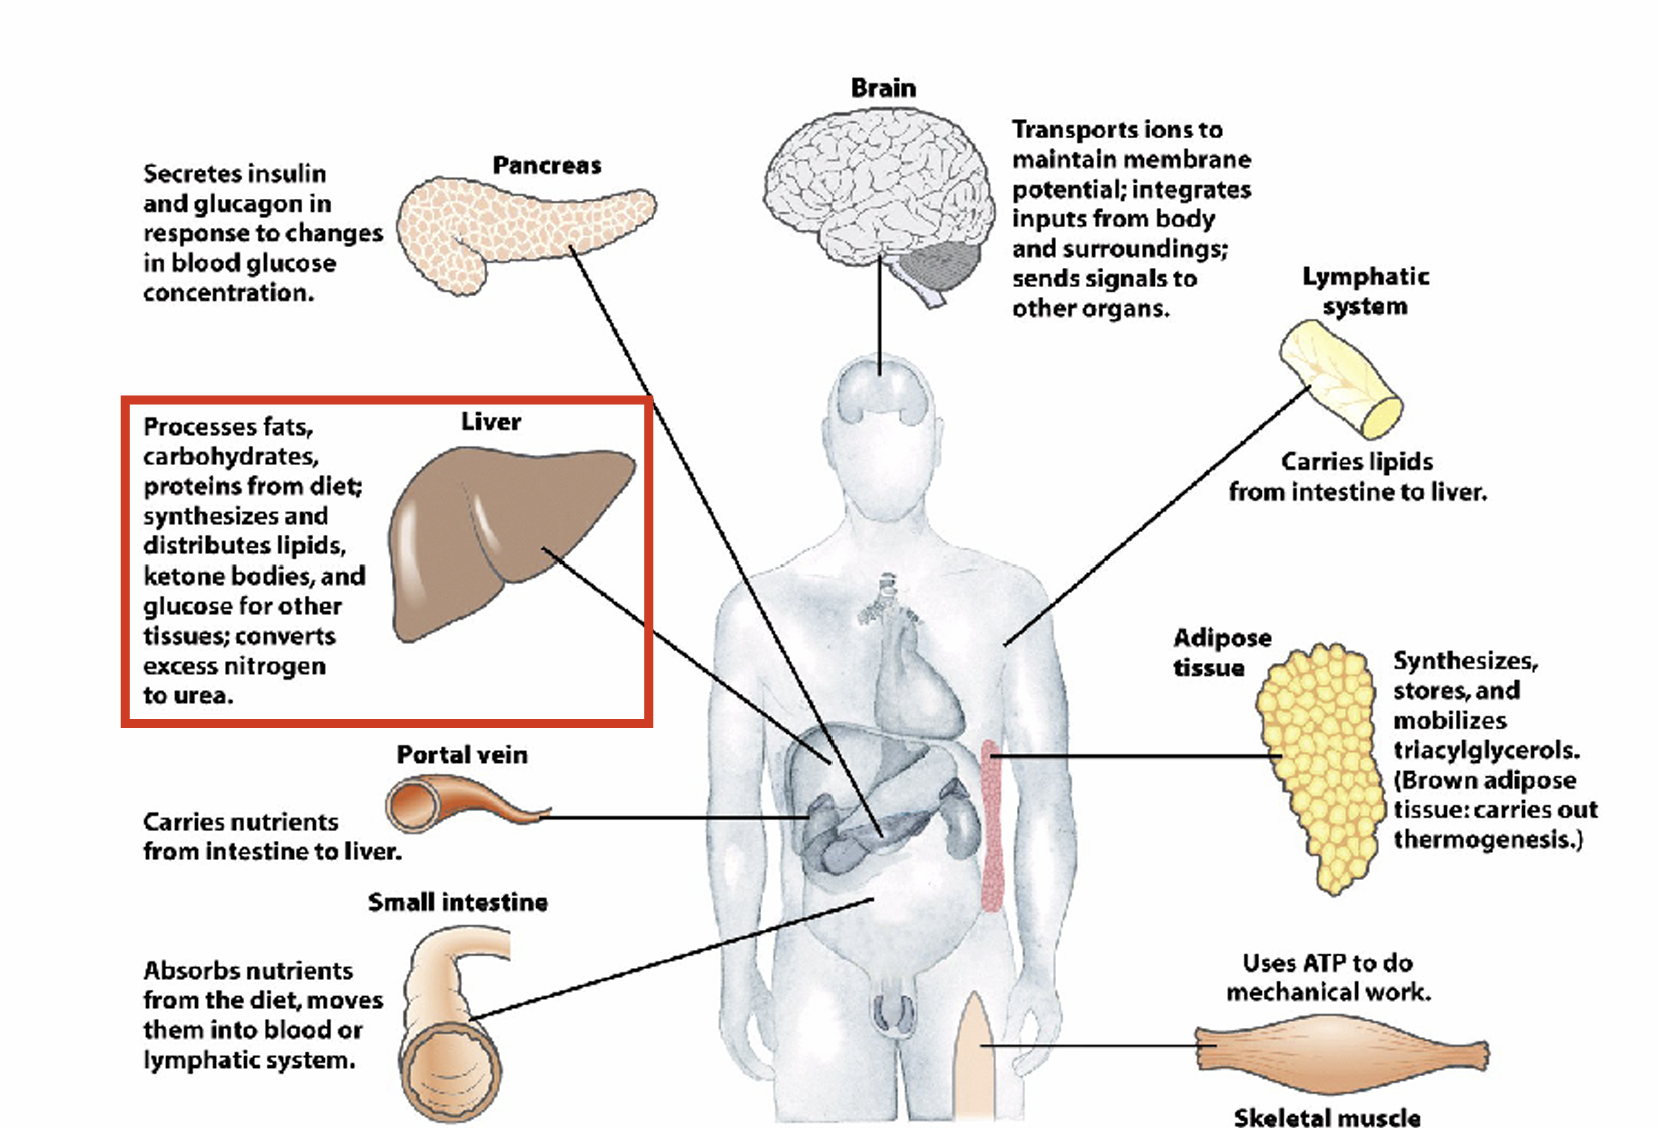
\includegraphics[width=\linewidth]{divisionLabour.png}
    \caption{division of labour of metabolism}
    \label{fig:enter-label}
\end{figure}
Not all cells are equally metabolically active. In fact some cells have totally different tasks in the metabolic pathways. 
(not much else here)

\subsection{The liver}
\begin{figure}[H]
    \centering
    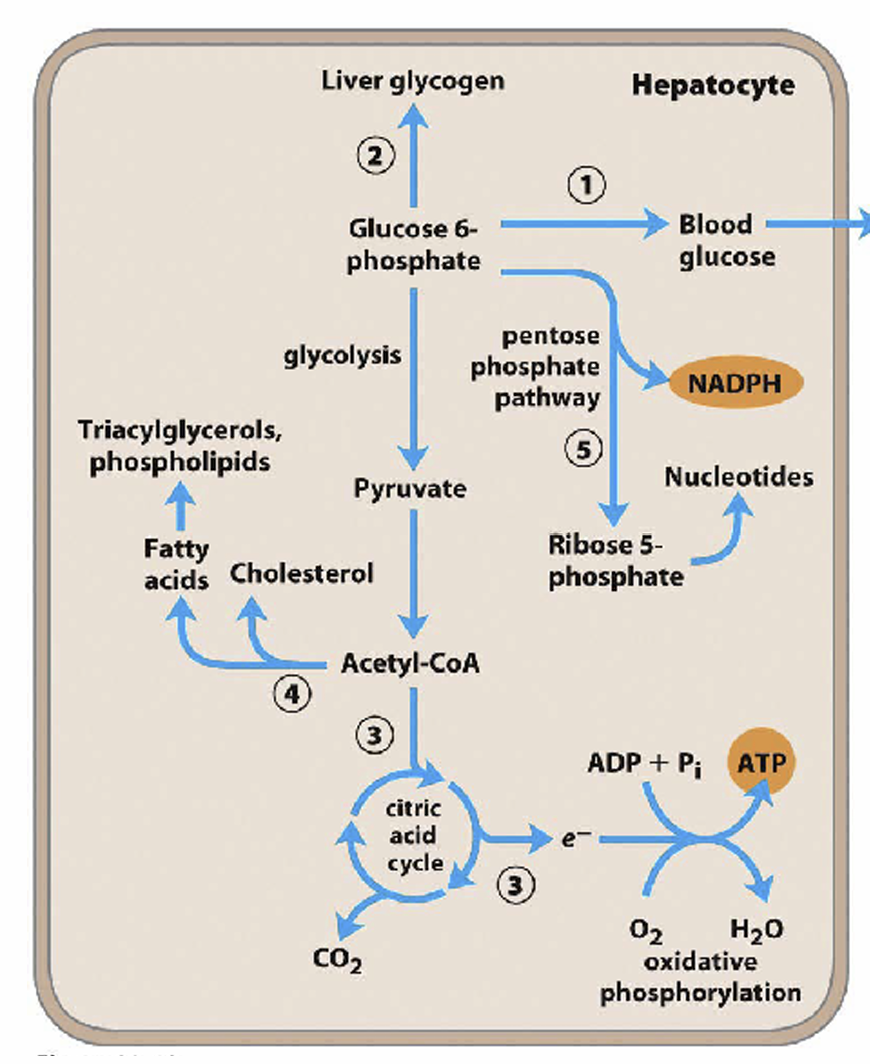
\includegraphics[width=0.5\linewidth]{Liver.png}
    \caption{Liver has various options to process Glucose 6 phosphate}
    \label{fig:enter-label}
\end{figure}
\subsubsection{glucose 6 phosphate processing}
When we eat sugar it is imported into the liver and converted to glucose 6 phosphate. The liver has many different things it \textbf{can do with glucose-6-phosphate}:
\begin{itemize}
    \item convert it back to glucose and export it into the blood stream ( this is a unique ability of the liver cells)
    \item make glycogen
    \item use it to make ATP via glycolysis TCA cylce and oxidative phophorylation
    \item make Acetyl-CoA after glycolysis to then make Fatty acids, triglycerols and Fatty acids.
    \item feed it to the pentose pathway (used for dNTP sythesis)
\end{itemize}
\paragraph{the pentose pathway}
\begin{figure}[H]
    \centering
    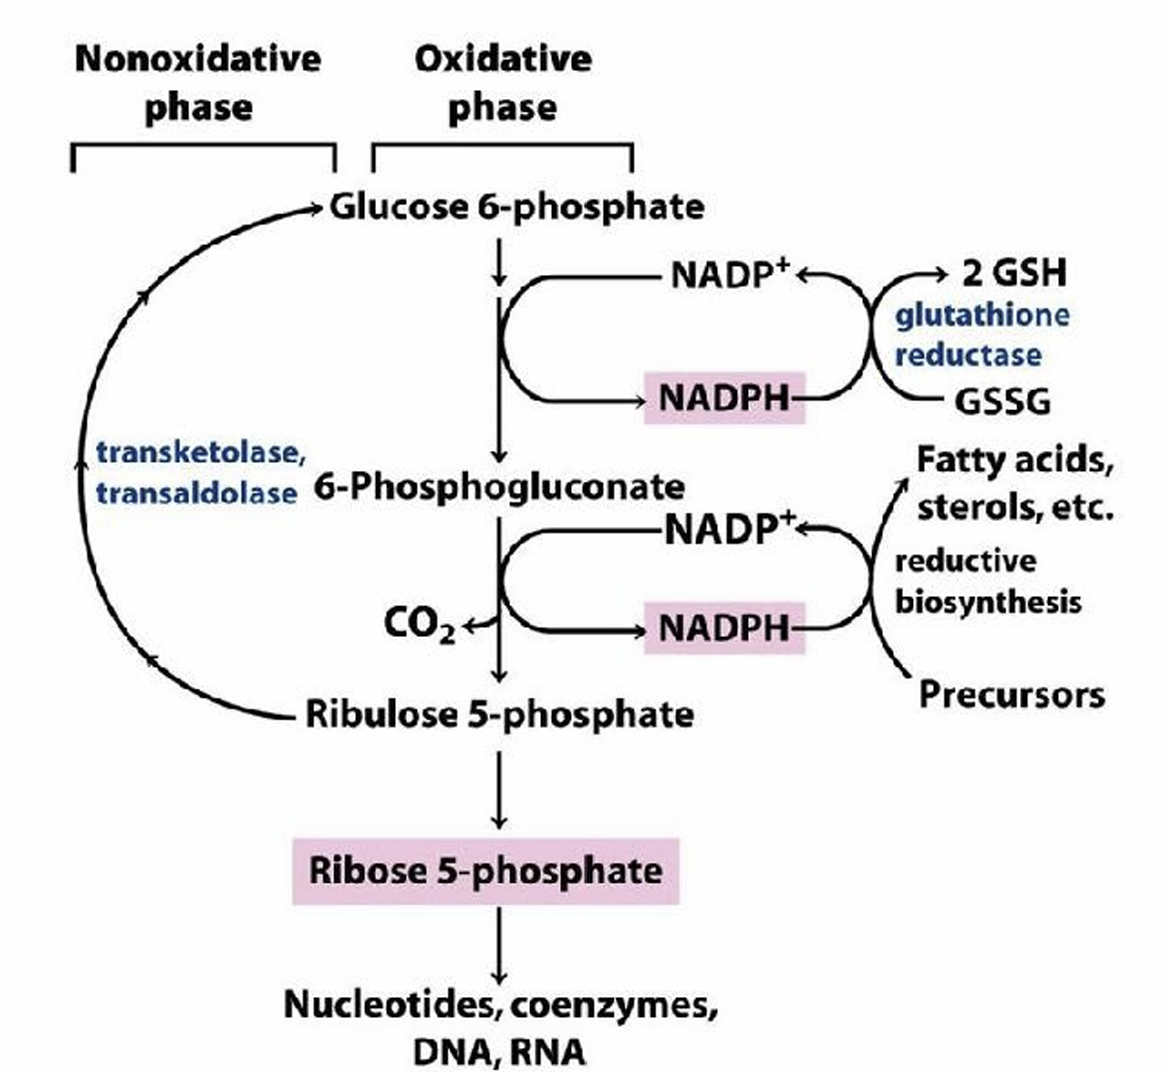
\includegraphics[width=0.5\linewidth]{PPP.png}
    \caption{pentose pathway}
    \label{fig:enter-label}
\end{figure}
This is a very short sumamry since we didn't cover this in detail but this pathway is used t\textbf{o produce nucleotides.} THis pathway is\textbf{ highly active in cancer cells,} which is a reason for the warburg effect. (cancer cells prefer glycolysis because they tend to have less oxygen and need more nucleotides to fuel their expanisve growth)
\subsubsection{amino acid processing}
\begin{figure}[H]
    \centering
    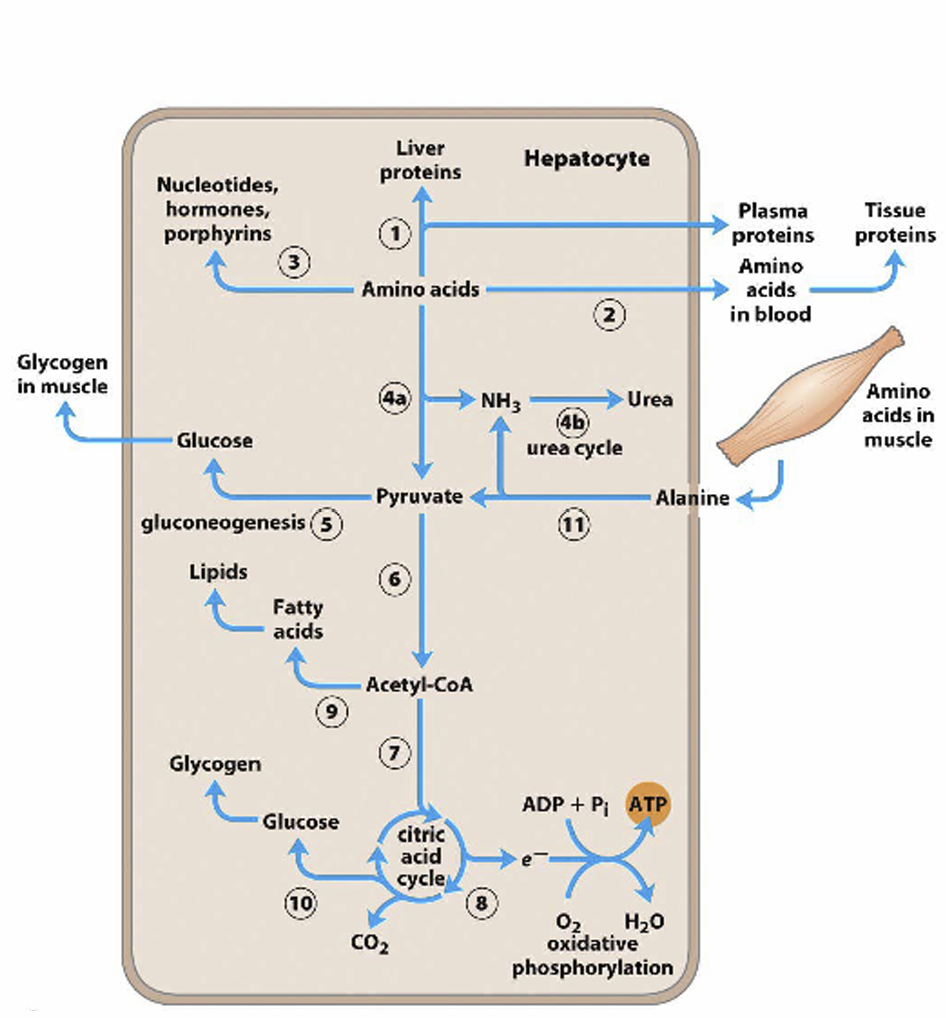
\includegraphics[width=0.5\linewidth]{liverAminoAcid.png}
    \caption{amino acid processing in the liver}
    \label{fig:enter-label}
\end{figure}
The liver is also the organ that is responsible for \textbf{processing amino acids}
\begin{itemize}
    \item used to make liver proteins
    \item mobilized to blood stream to go somewhere else
    \item produce nucleotides hormones 
    and porphyrines 
    \item deanimated. amine group is turned to urea via the urea pathway
    \item rerouted to lipid or glucose metabolism (not favored)
    \item used to produce ATP (not favored)
\end{itemize}

\subsubsection{Lipid processing}
\begin{figure}[H]
    \centering
    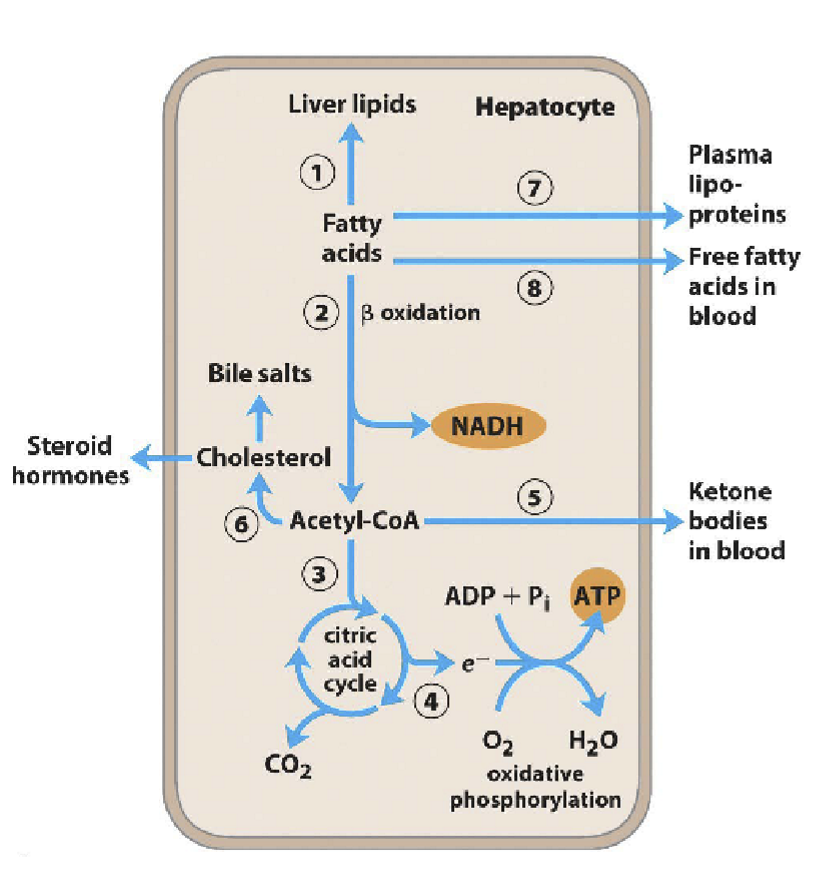
\includegraphics[width=0.5\linewidth]{liverLipids.png}
    \caption{lipid processing in the liver}
    \label{fig:enter-label}
\end{figure}
the liver has many possibilites to process liver cells:
\begin{itemize}
    \item used to produce lipids that the liver itself needs
    \item use $\beta$-oxidation to produce Acetyl-CoA:
    \begin{itemize}
        \item feed Acetyl-CoA into TCA cycle to produce ATP
        \item use it to \textbf{make keton bodies}
        \item use it to make sterols like \textbf{cholesterol}
    \end{itemize}
    \item Fatty acids can be mobilised 
    through the blood stream either as 
    phospholipids/ triglycerides bound to 
    lipoproteins or as free fatty acids bound 
    to albumim
\end{itemize}
\paragraph{keton bodies}
\begin{figure}[H]
    \centering
    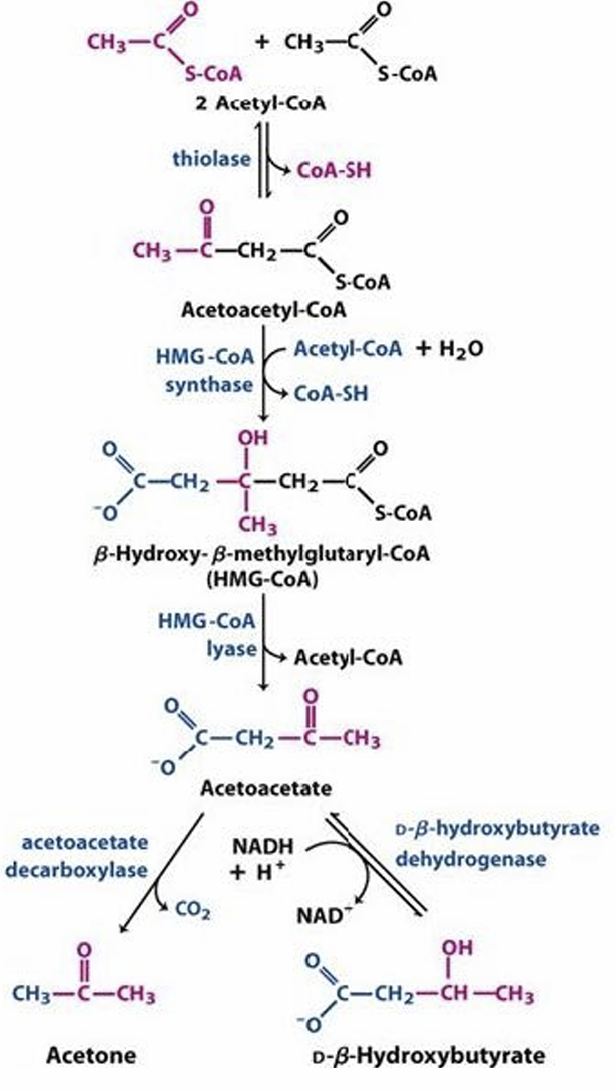
\includegraphics[width=0.3\linewidth]{ketonBodies.png}
    \caption{keton bodies production}
    \label{fig:enter-label}
\end{figure}
keton bodies are produced during \textbf{starvations carbohydrate 
restrictive diets, prolonged intense 
exercise, alcoholism, or in untreated (or 
inadequately treated) type 1 diabetes mellitus. }. These are readily transported to the body and \textbf{converted to acteyl-CoA} which can be fed into the TCA cycle to produce ATP. \textbf{In the brain they can be used to make long fatty acid chains.}

\subsection{The muscles}
\begin{figure}[H]
	\centering
	\subfigure[cori cycle]{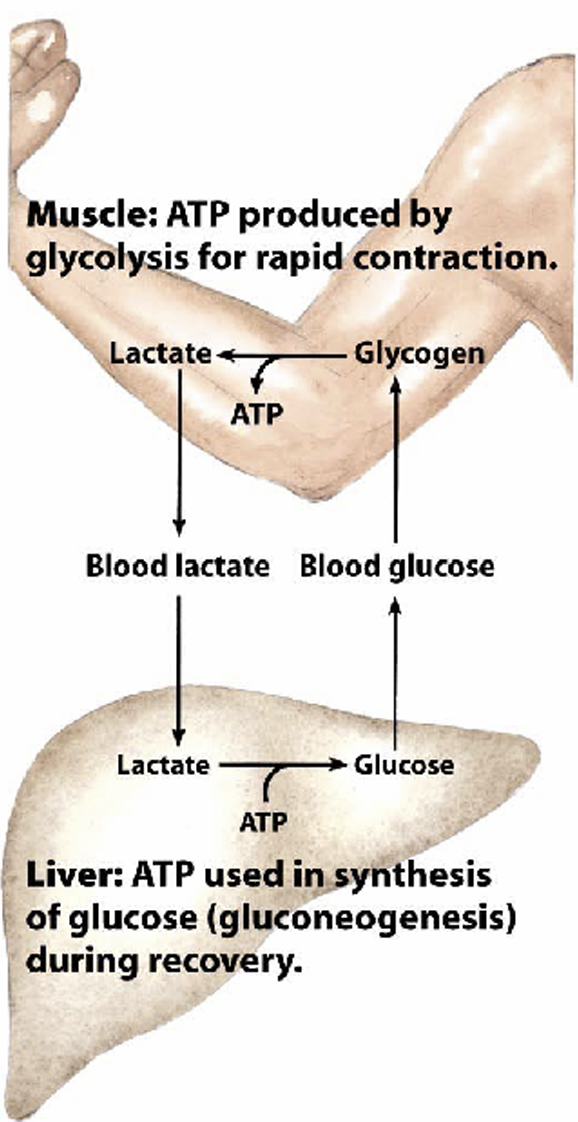
\includegraphics[width = 0.2\textwidth]{muscle.png}}
	\subfigure[muscle metabolism]{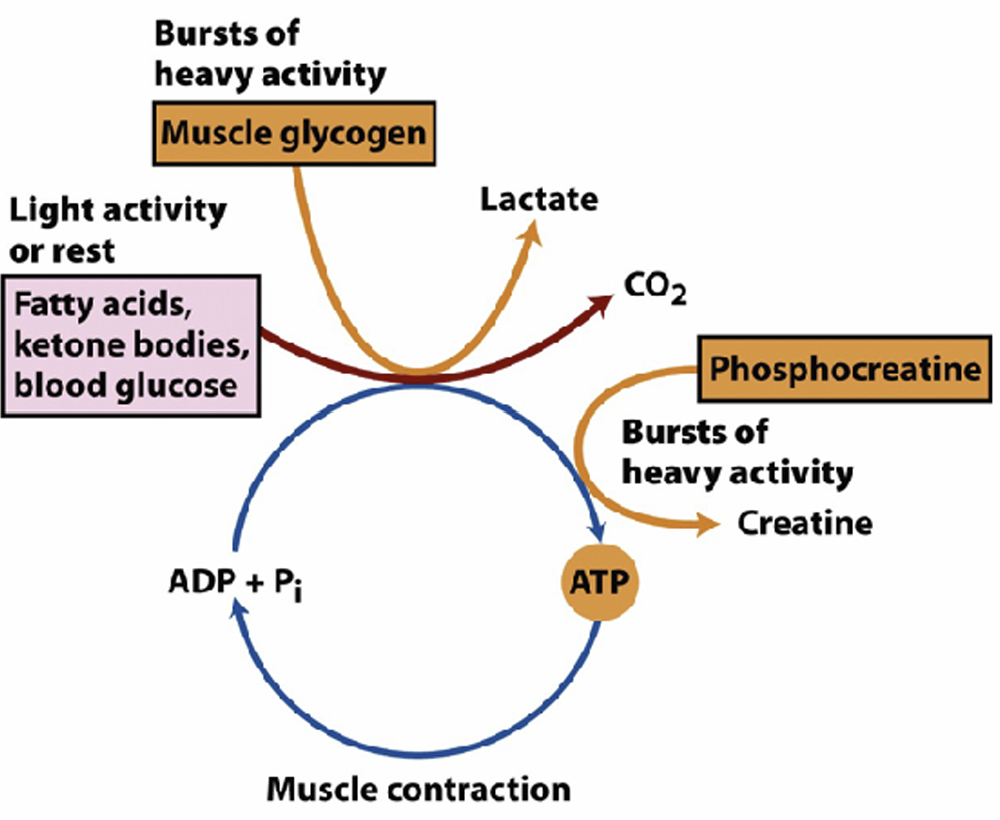
\includegraphics[width = 0.5\textwidth]{muscleMetabolism.png}}
	\caption{muscle metabolism}
\end{figure}
The muscle cells consume around\textbf{ 50\% of the bodies ATP} at rest (\textbf{during exercise it's 90\%}). Muscle cells use different energy sources depending on the activity level due to issues with replenishment:
\begin{itemize}
    \item under resting conditions: use glucose, keton bodies and fatty acids
    \item during heavy prolonged exercise: use glycogen storages and make ATP via \textbf{lactic fermentation}
    \item for heavy short bursts of energy the muscles can use phosphocreatine.
\end{itemize}
The \textbf{\gls{cori-cycle}} is at the heart of why you're muscles heart like shit after sport. The liver produces glucose that reaches the muscles, these then use it for ATP and produce lactate, which is transported to the liver to be broken down.

\subsection{The brain}
\begin{figure}[H]
    \centering
    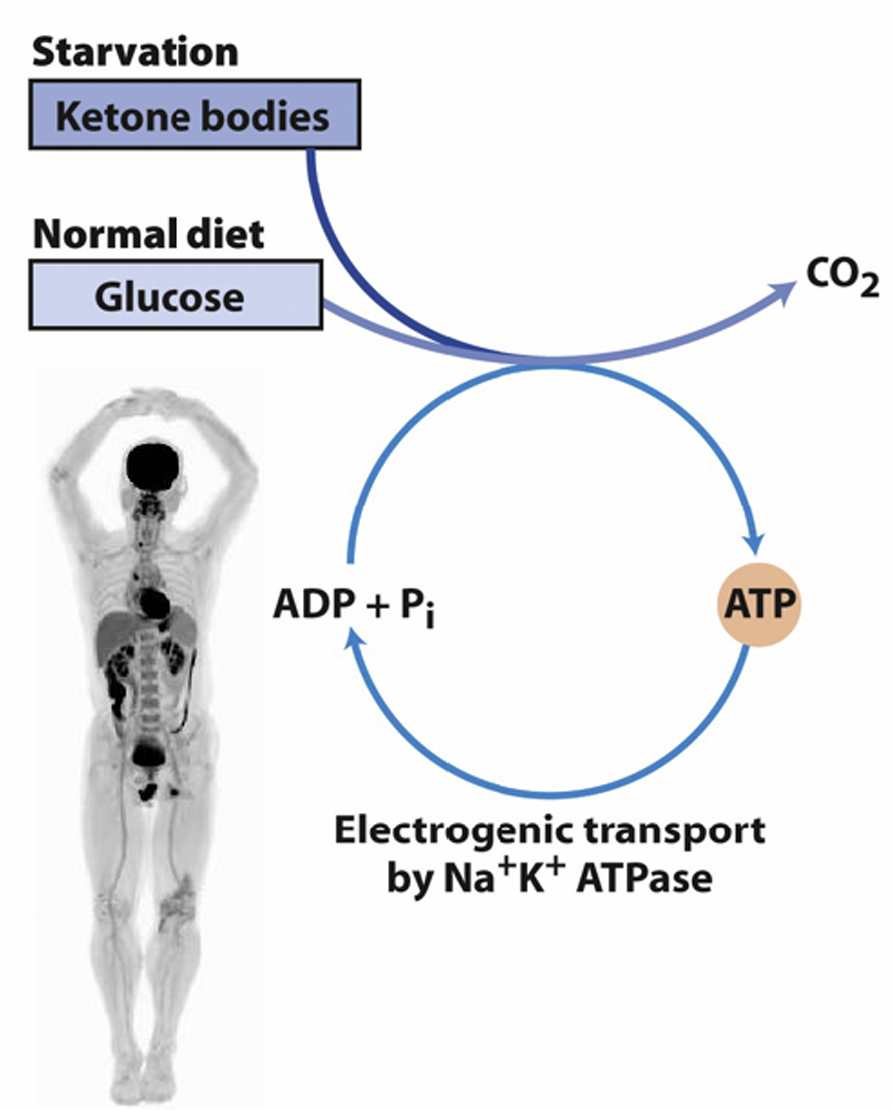
\includegraphics[width=0.5\linewidth]{theBrain.png}
    \caption{the brain consumues an insane amout of glucose}
    \label{fig:enter-label}
\end{figure}
The brain is responsible for 20\% of the total oxygen consumtion, due to it's high energy demand. This is because it almost\textbf{ exclusively uses glucose and keton bodies for ATP production.} It has very little glycogen storage so is highly dependent on the blood glucose levels being high enough ( so eat bread my friends..)
\subsection{Adipose tissue}
\begin{figure}[H]
    \centering
    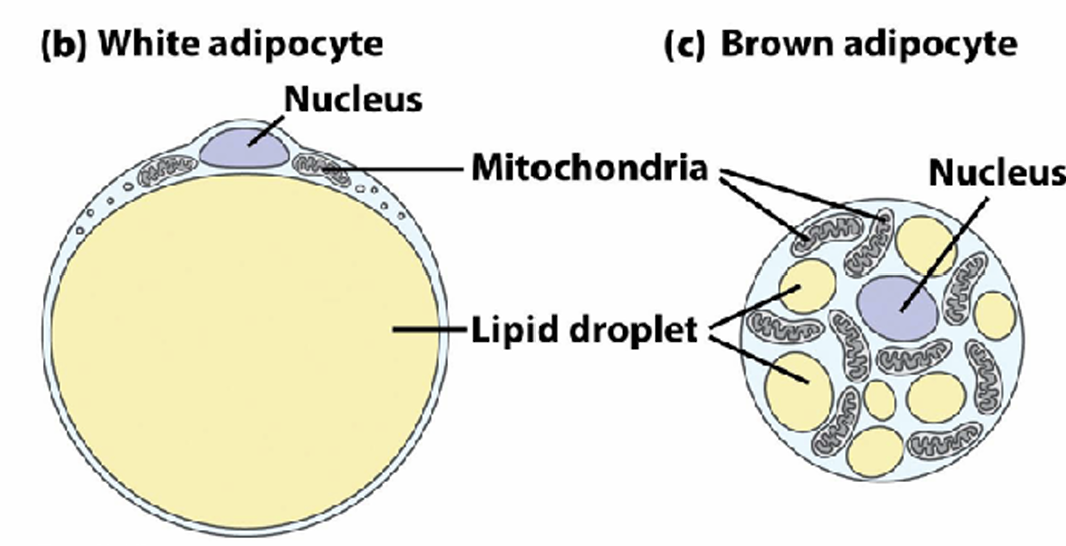
\includegraphics[width=0.5\linewidth]{adiposeTissue.png}
    \caption{two types of Adipose tissue}
    \label{fig:enter-label}
\end{figure}
Adipocytes are cells that are responsible for storing Fatty acids for energy use aswell as thermal insulation of the body. There are \textbf{two types white adipocytes whose main role is to store fatty acids and brown adipocytes which generate heat} Free floating fatty acids need to be transported around the blood steam by lipoproteins. Once they reach the adipose tissue they are cleaved from the lipoprotein by \textbf{\gls{lipoprotein-lipase}}


\subsection{the Pancreas}
\begin{figure}[H]
    \centering
    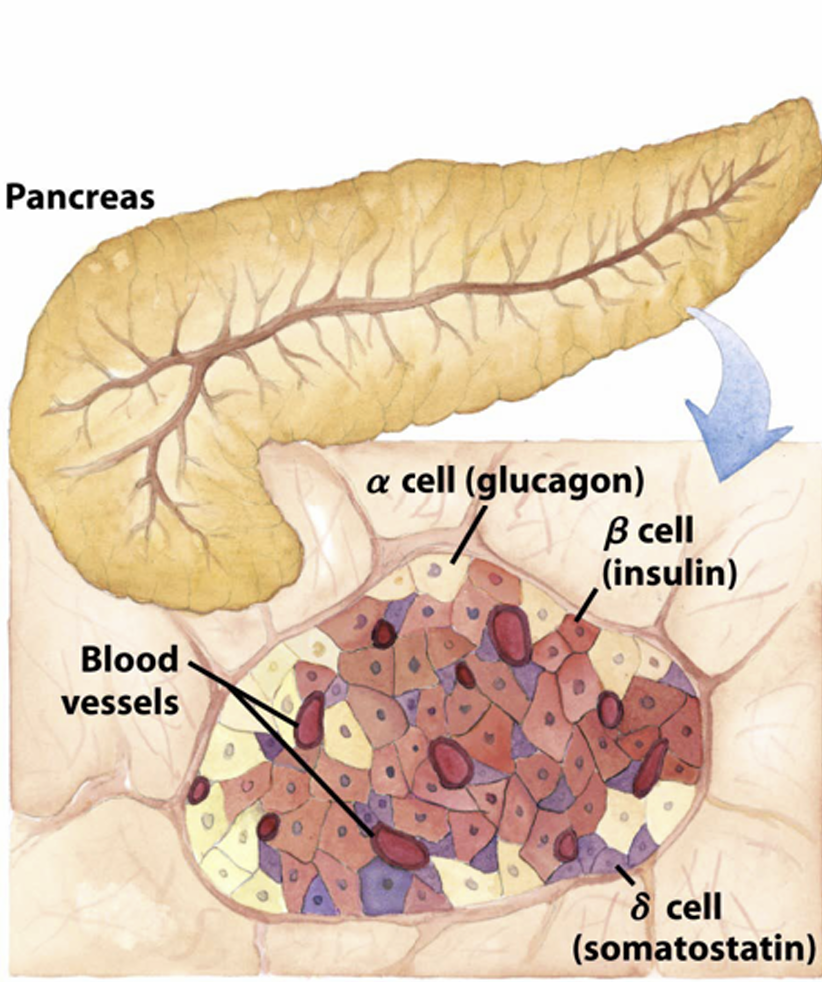
\includegraphics[width=0.5\linewidth]{pancreas.png}
    \caption{pancreas and langerhas islets}
    \label{fig:enter-label}
\end{figure}
The pancreas is a super imporntant organ for\textbf{ blood sugar level regualtion.} In the pancreas there are \textbf{langerhans islet }which consist of $\alpha$-cells $\beta$-cells $\delta$-cells. These are well connected with the cardio vascular system to deliver their hormones everywhere. These islets secrete insulin and glucagon: \textbf{$\alpha$-cells  produce glucagon and $\beta$-cells insulin}.

\subsection{the blood}
\begin{figure}[H]
	\centering
	\subfigure[blood composition]{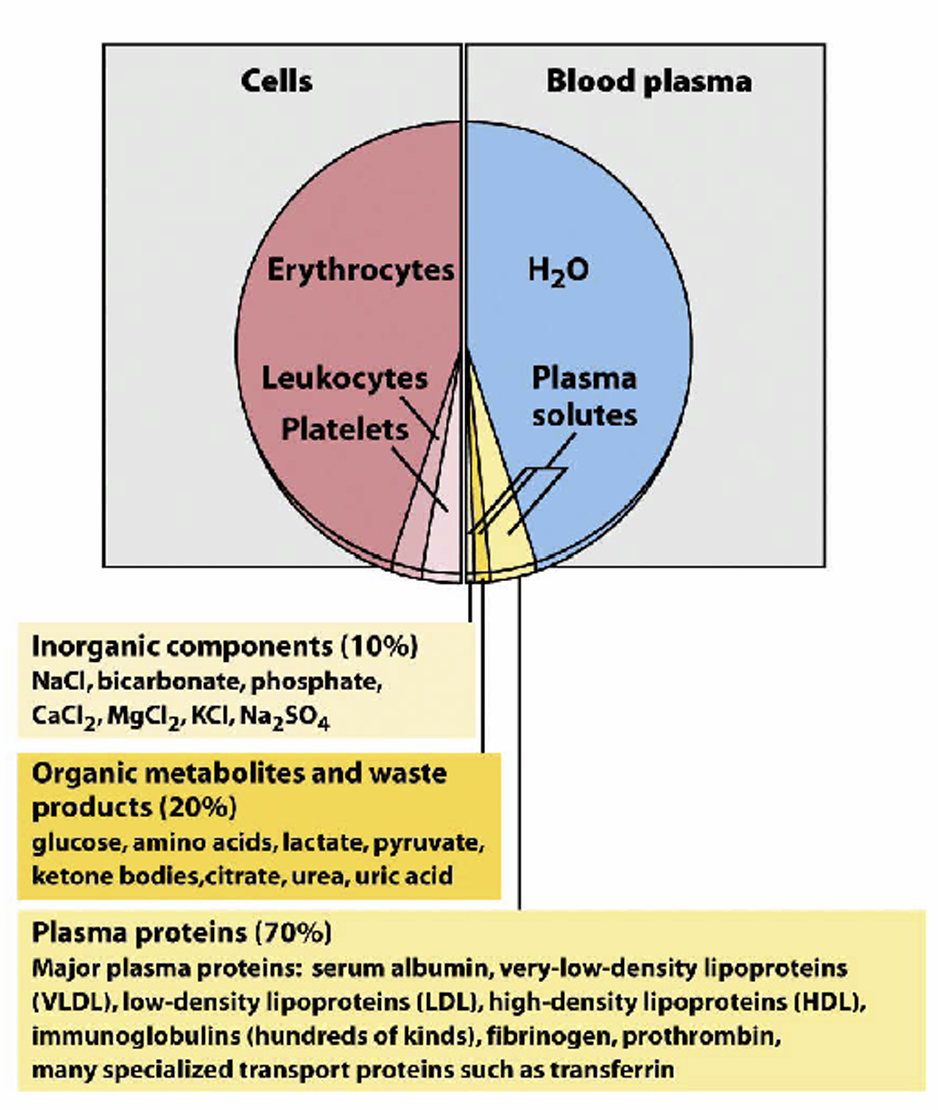
\includegraphics[width = 0.4\textwidth]{bloodComposition.png}}
	\subfigure[glucose levels in blood]{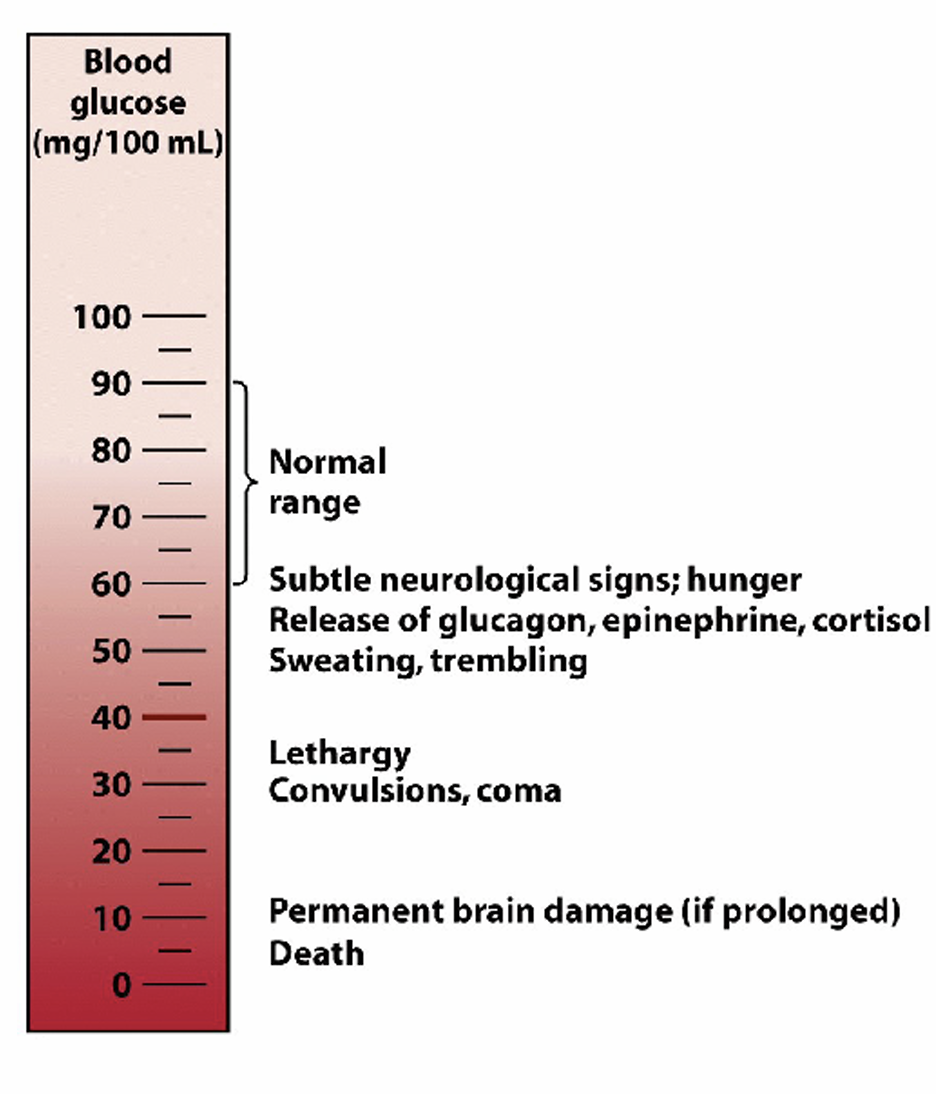
\includegraphics[width = 0.4\textwidth]{glucoseLevels.png}}
	\caption{the blood overview}
\end{figure}
The blood is responsible for \textbf{transporting everything throught the body} In the context of metabolism it's main role is to \textbf{distribute glucose} to all the cells in the body, as well as \textbf{transport hormones }so that the cells can respond accordingly.

When there isn't enough sugar in the blood \textbf{(below 2.2 mM or 40 mg/dL)} the body is in a state of \textbf{\gls{hypoglycemia}}, This can have various not so good consequences and if prolonged will lead to permanent brain damage or even death.


\subsection{neuro endocrine system}
\begin{figure}[H]
    \centering
    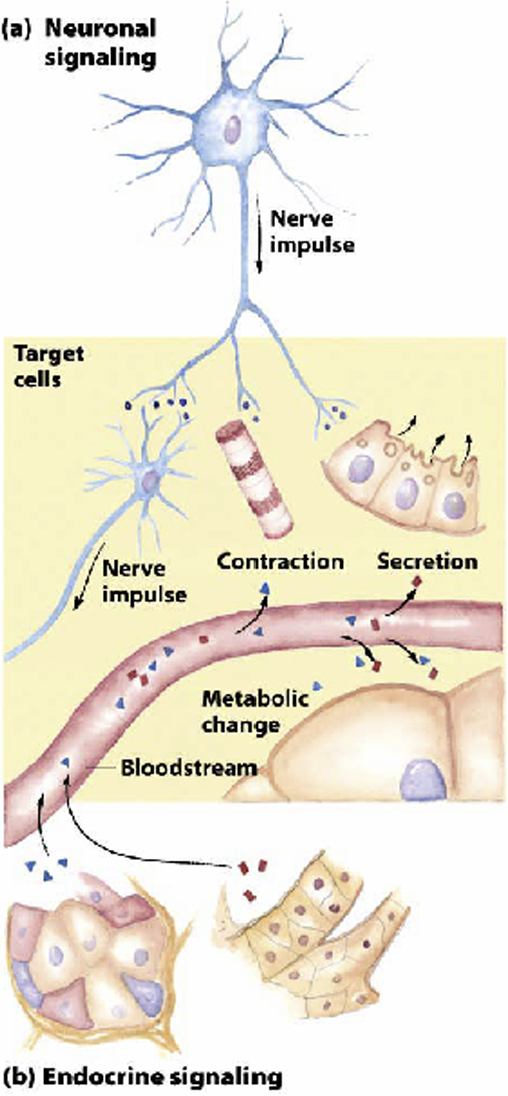
\includegraphics[width=0.3\linewidth]{NeuroEndocrineSystem.png}
    \caption{Enter Caption}
    \label{fig:enter-label}
\end{figure}
Neurons act locally via neurotransmitters, which can only act at very small distances and generally have very specific responses. Hormones on the other hand travel long distances and trigger can trigger diverse responses in different organs. Through neuroendocrine integration, n\textbf{euroendocrine cells convert neuronal input into hormonal output to coordinate body functions.}
\subsubsection{types of hormones}
\begin{itemize}
    \item \textbf{Peptide hormones}: Made of a chain of amino acids, ranging from just 3 to hundreds.
    \item \textbf{Amino acid hormones}: Derived from amino acids, most commonly tyrosine.
    \item \textbf{Eicosanoid hormones}: Derived from lipids such as arachidonic acid.
    \item \textbf{Steroid hormones}: Derived from cholesterol.
\end{itemize}
\subsubsection{signal transduction}
\begin{figure}[H]
    \centering
    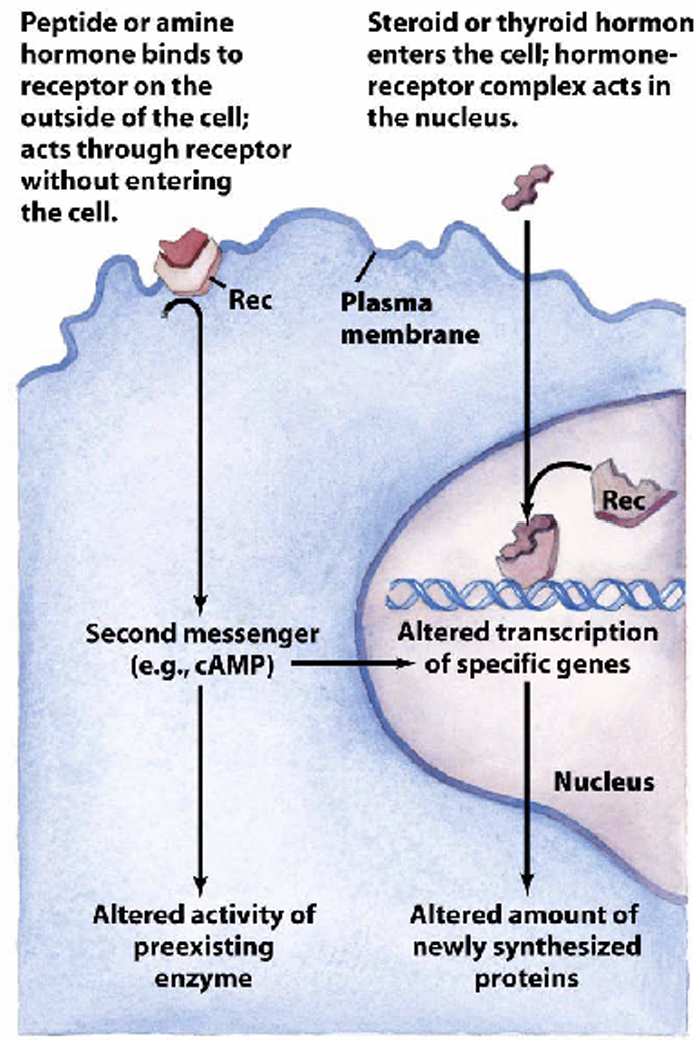
\includegraphics[width=0.3\linewidth]{signalTransduction.png}
    \caption{signal transduction}
    \label{fig:enter-label}
\end{figure}
\textbf{Hormones} act by binding to \textbf{receptor proteins}, triggering a \textbf{signal transduction pathway} that leads to \textbf{gene transcription} or faster responses like \textbf{phosphorylation of effector proteins} and \textbf{membrane trafficking}. 

\textbf{Effector proteins} are molecules that carry out the cellular response to a signal, such as enzymes or ion channels. They are often regulated by phosphorylation. This type of signal transduction is much faster than via transcription factors.
\subsubsection{the endocrine system's main players and heirarchy}
\begin{figure}[H]
    \centering
    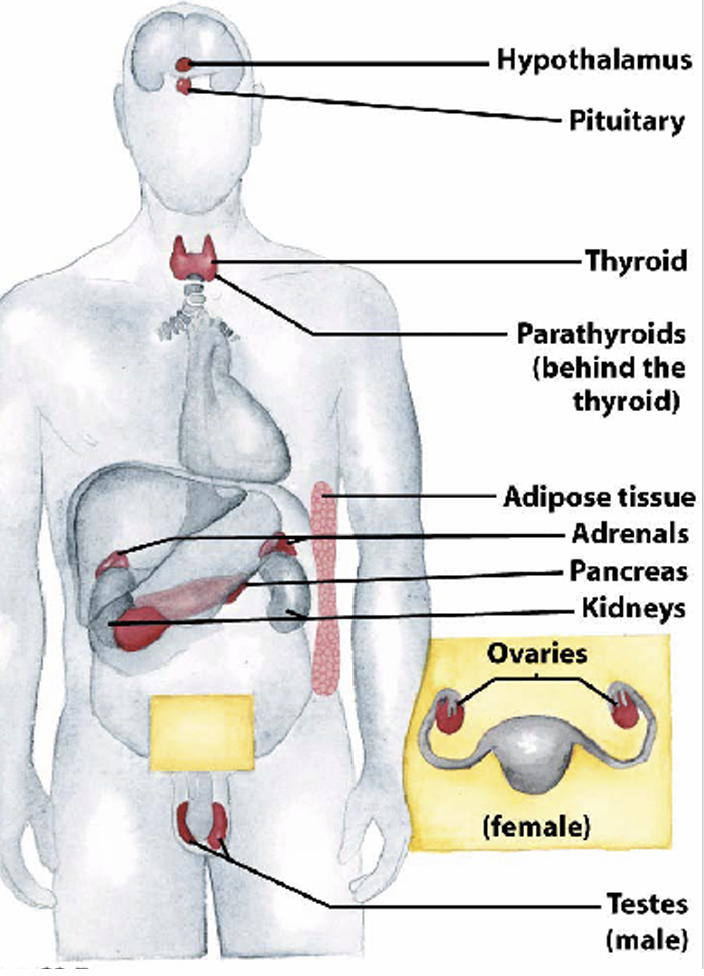
\includegraphics[width=0.3\linewidth]{endocrineSystem.png}
    \caption{main organs in endocrine system}
    \label{fig:enter-label}
\end{figure}
\begin{itemize}
    \item \textbf{\gls{hypothalamus}}: Produces hormones that target the anterior pituitary and sends neuronal signals to the posterior pituitary in response to nervous system stimuli.
    
    \item \textbf{\gls{anterior-pituitary}}: Produces hormones that target downstream endocrine organs including the adrenal cortex, thyroid, testes, and ovaries in response to signals from the hypothalamus.
    
    \item \textbf{\gls{posterior-pituitary}}: Contains axons of neurons whose cell bodies reside in the hypothalamus. These neurons secrete \gls{oxytocin} and \gls{vasopressin}.
    
    \begin{itemize}
        \item \textbf{\gls{oxytocin}} targets smooth muscle in the uterus and mammary glands to induce labor and lactation.
        \item \textbf{\gls{vasopressin}} regulates blood pressure.
    \end{itemize}
\end{itemize}
These organs are usually organized in a hierarchy with the hypothalamus calling the shots and telling the rest of the organs what to do.
\begin{figure}[H]
    \centering
    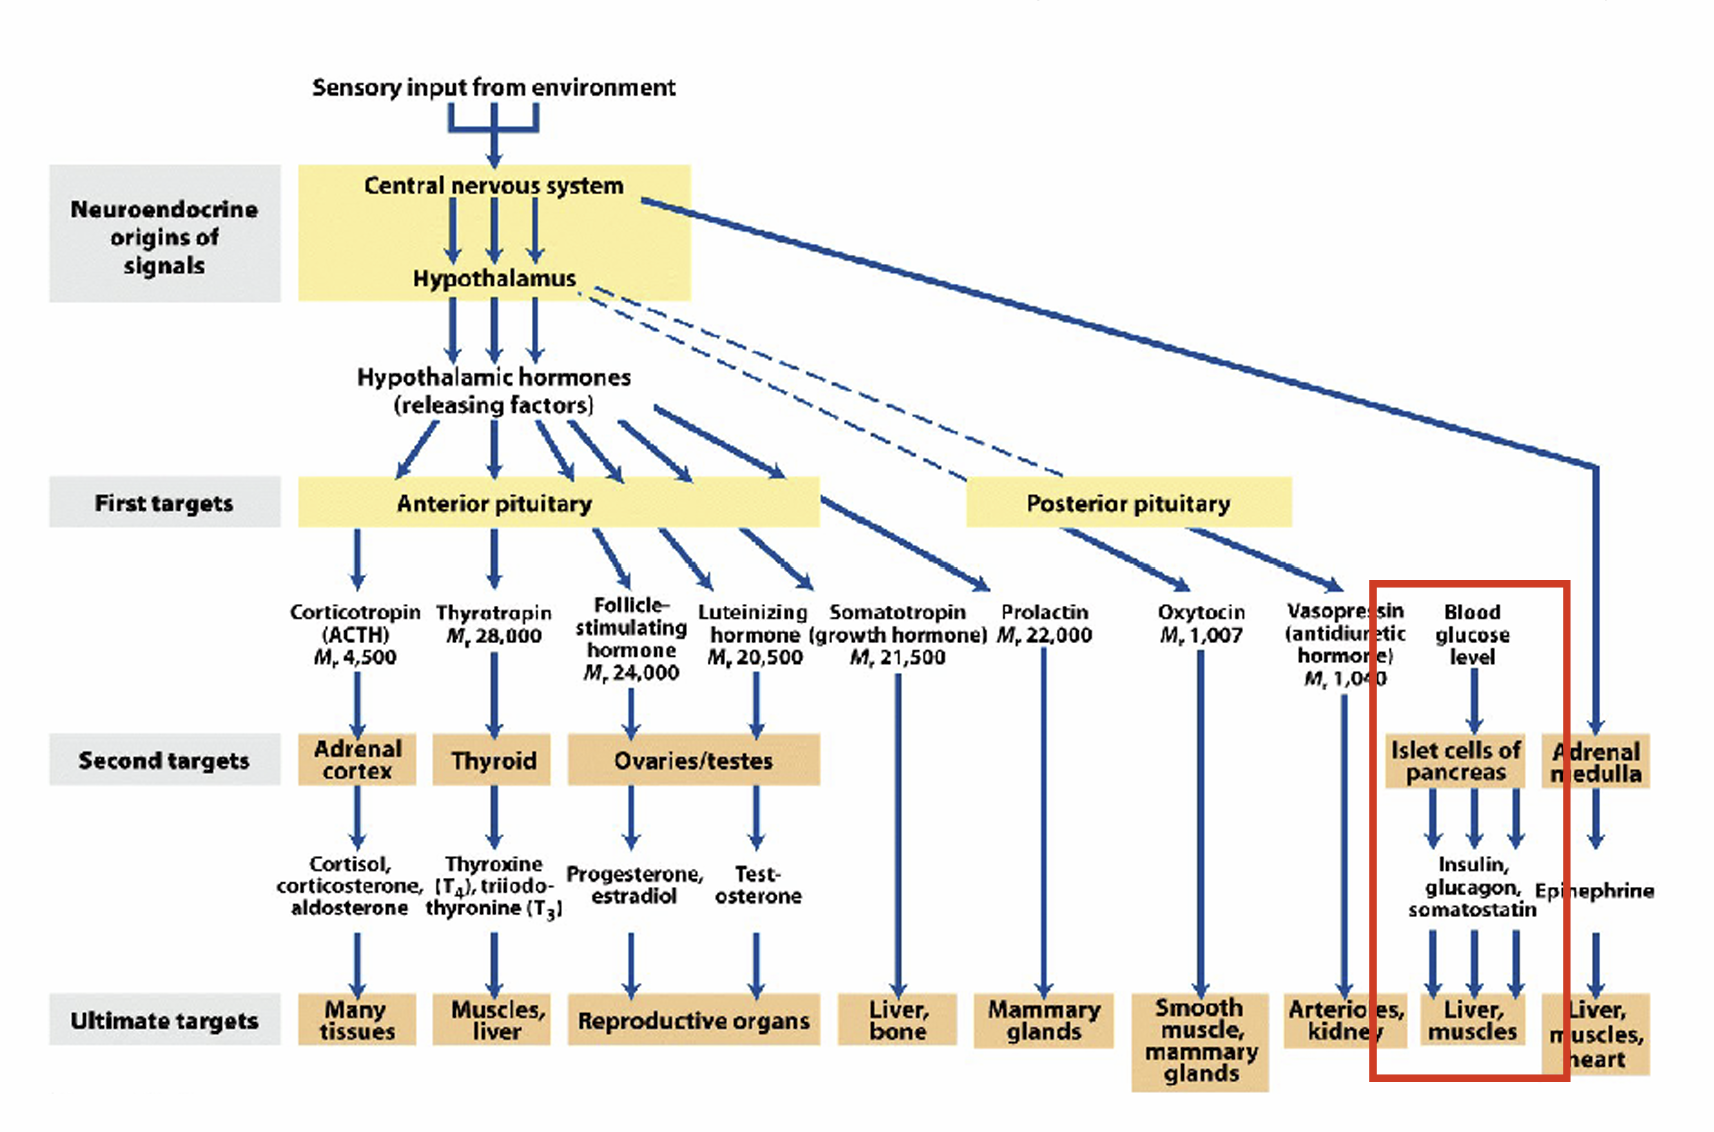
\includegraphics[width=0.5\linewidth]{heirarchy.png}
    \caption{hierarchy of the neuroendocrine system}
    \label{fig:enter-label}
\end{figure}
\subsection{blood glucose regulation}
\begin{figure}[H]
    \centering
    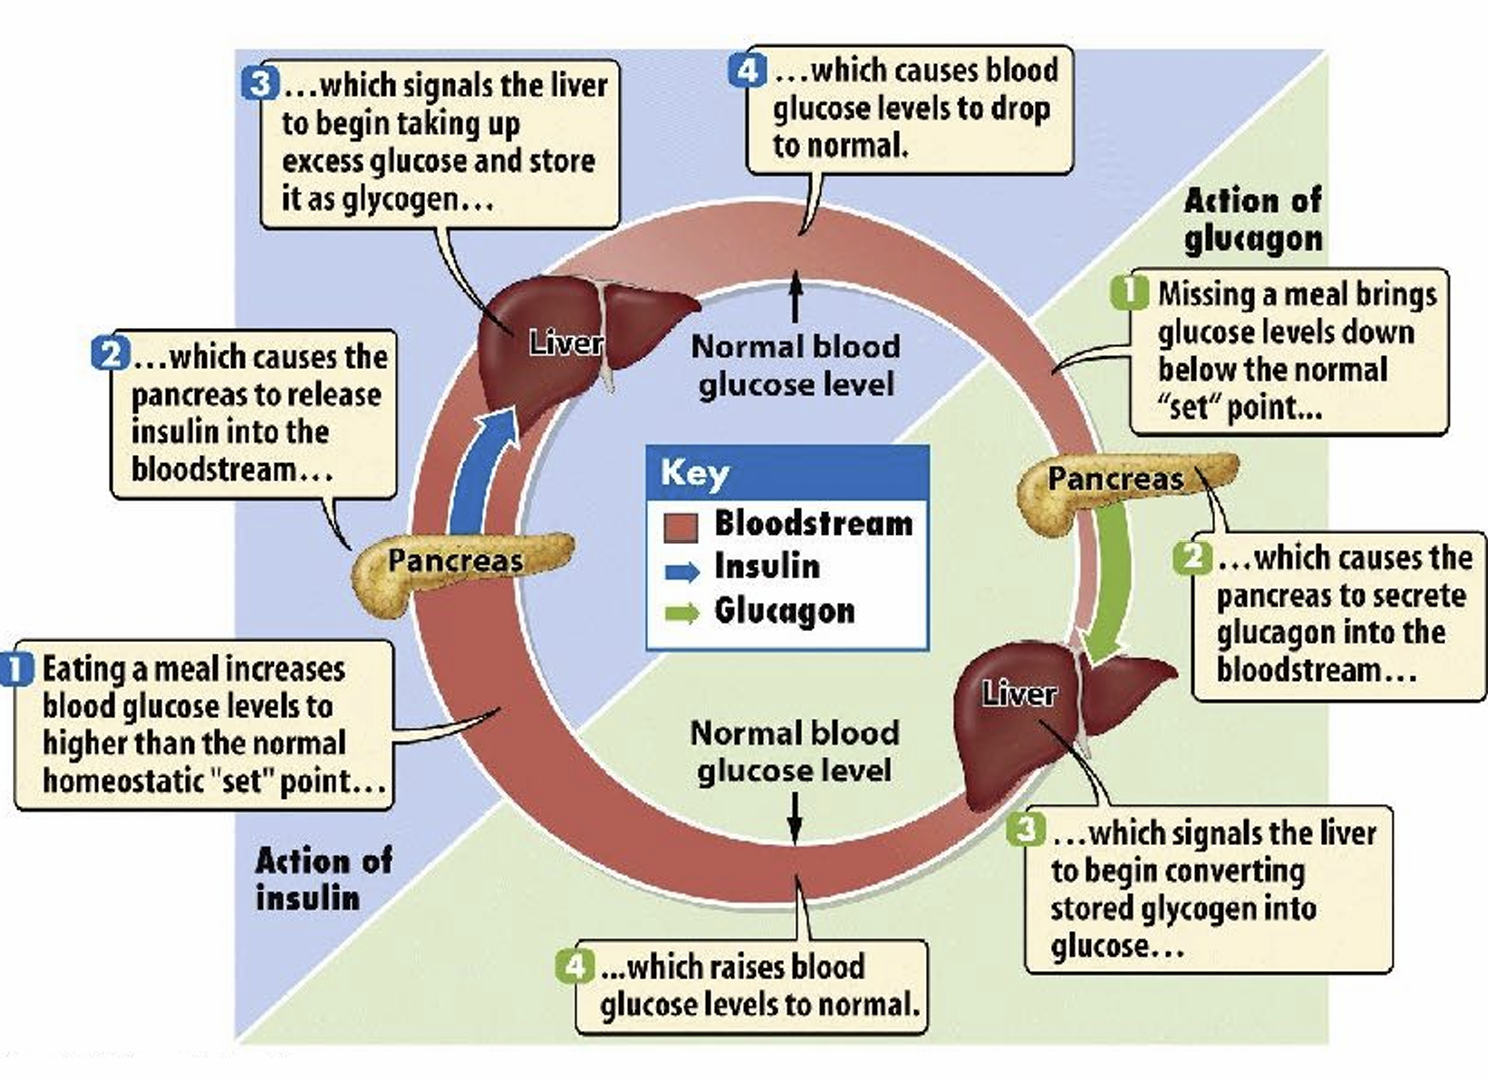
\includegraphics[width=0.5\linewidth]{bloodSugarRegulation.png}
    \caption{blood sugar regulation}
    \label{fig:enter-label}
\end{figure}
Blood sugar regulation happens primarily via two \textbf{enzymes insulin and glucagon}. 
\begin{itemize}
    \item insulin: insulin is used to lower the blood sugar level
    \item glucagon: is used to raise the blood sugar level.
\end{itemize}
\subsubsection{beta cells}
\paragraph{insulin release mechanism}
\begin{figure}[H]
    \centering
    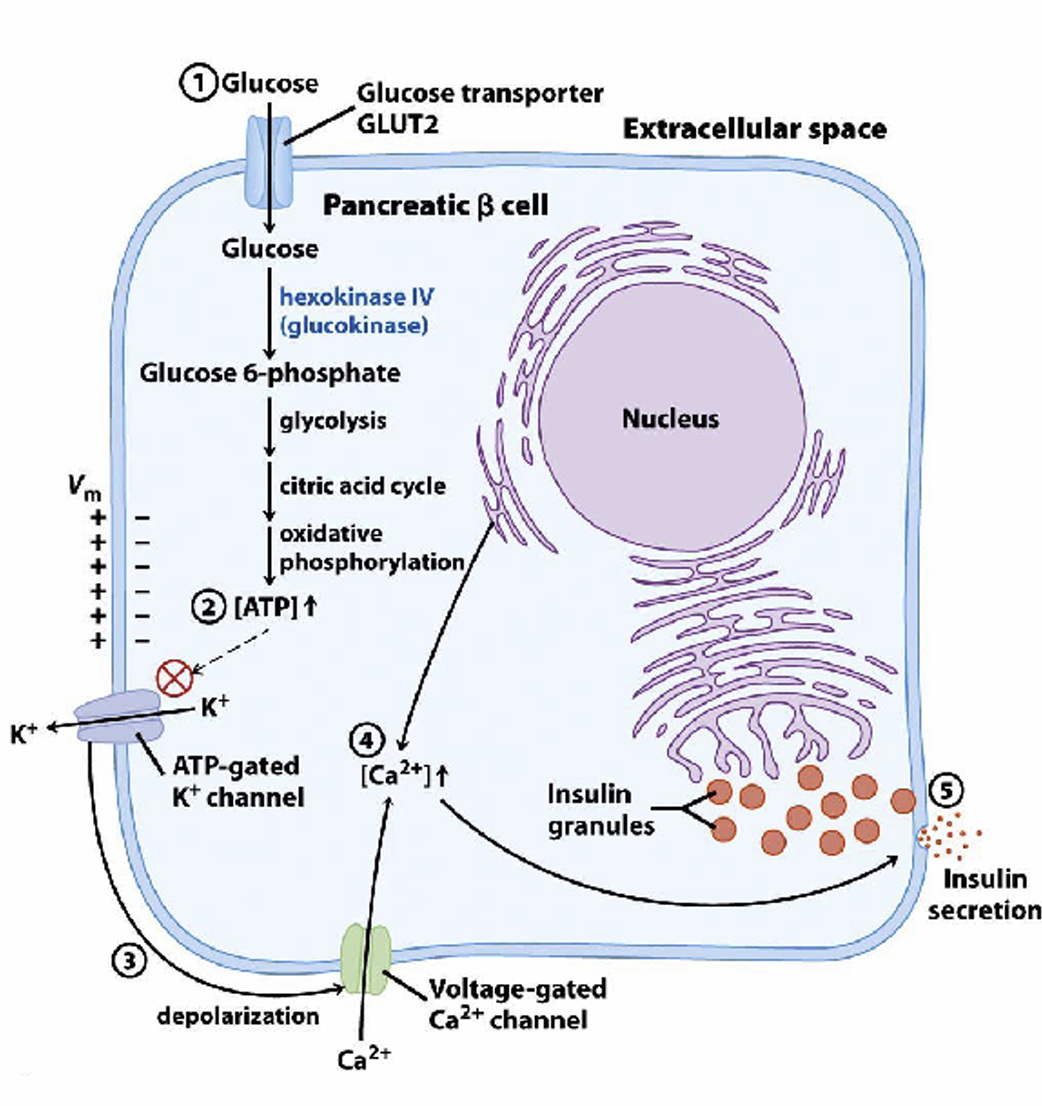
\includegraphics[width=0.5\linewidth]{betaCells.png}
    \caption{insulin function}
    \label{fig:enter-label}
\end{figure}
glucose enters $\beta$-cells via \textbf{glut2 glucose transporter}. This will then be used to \textbf{create ATP}. this is how the cells measure the glucose transportation in the blood. when there is too much glucose in blood:
\begin{enumerate}
    \item high ATP concentration inhibits ATP-gated K+ channels
    \item This will cause the membrane to depolarize, which will\textbf{ activate a ca2+ voltage gated channels. }
    \item the \textbf{influx of calcium} into the cell from the outside aswell as the ER, will cause the fusion of insulin granues to fuse with the membrane and be released via the \textbf{\gls{snarecomplex}}
\end{enumerate}
\paragraph{$\beta$-cells K-ATP channels}
\begin{figure}[H]
    \centering
    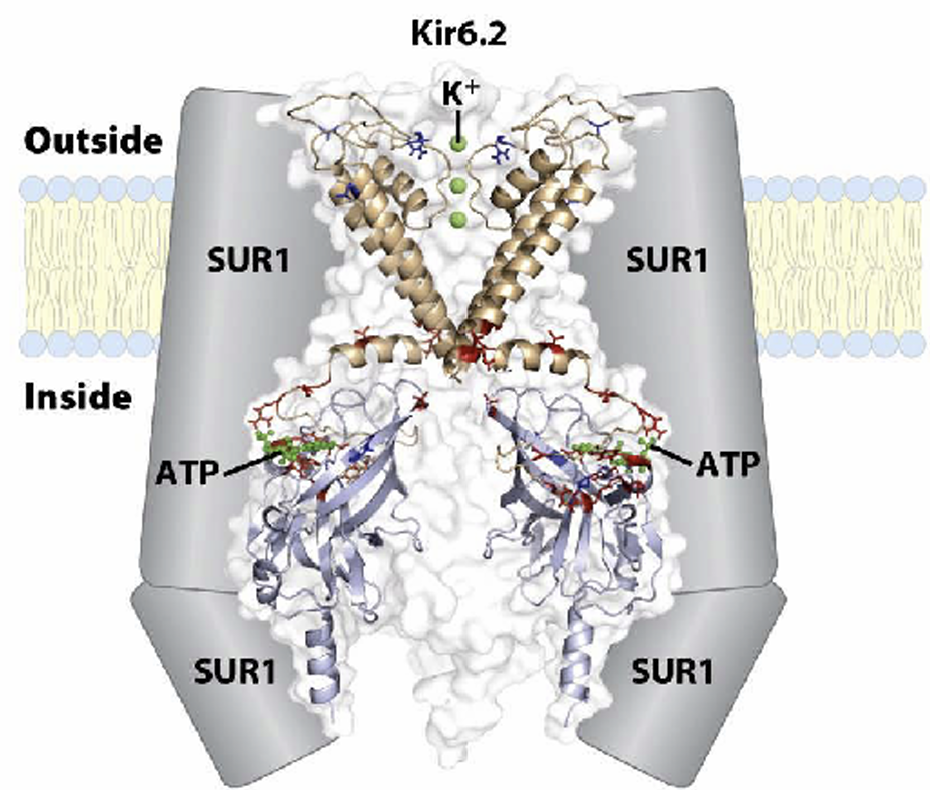
\includegraphics[width=0.5\linewidth]{KATPCHannel.png}
    \caption{KATP channels}
    \label{fig:enter-label}
\end{figure}
\textbf{\gls{katpchannel}} are regulated by the receptor sulphonylurea (\textbf{\gls{sur}}1), of which it has 4. It ha\textbf{ 4 pore forming K+ channels}. ATP inhibits KATP 
channels at the \textbf{Kir6.2 subunit}. Some \textbf{anti-diabetic sulphonylurea drugs work by interacting with SUR1 }
through an interaction with SUR1, to stimulate insulin secretion.
\paragraph{SNARE vesicle fusion}
\begin{figure}[H]
    \centering
    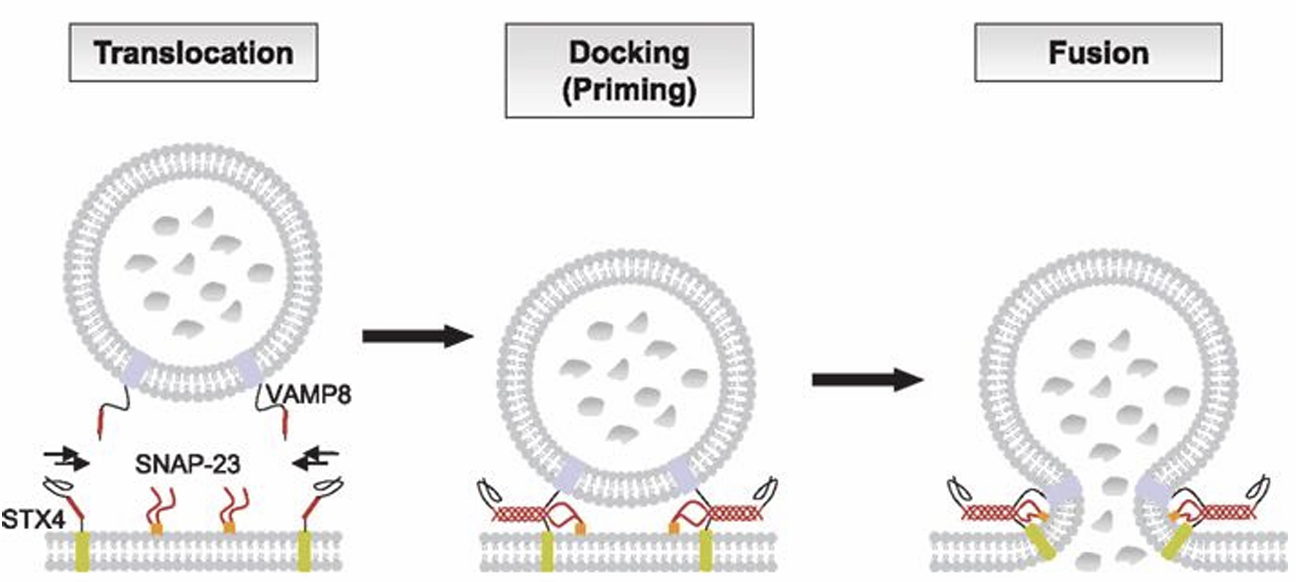
\includegraphics[width=0.5\linewidth]{snare.png}
    \caption{SNARE vesicle fusion }
    \label{fig:enter-label}
\end{figure}
The type of snare protein on the granules is \textbf{\gls{synaptobrevin2}}. and the membrane bound SNARE \textbf{\gls{syntaxin1a} in a complex with SNAP-25}.  \textbf{\gls{synaptotagmin}} is used to control insulin granule fusion through the concentration of ca2+. Upon exposure to Calcium this protein will \textbf{bind the Syntaxin1A-Synaptobrevin2 pair}

\paragraph{insulin production}
\begin{figure}[H]
    \centering
    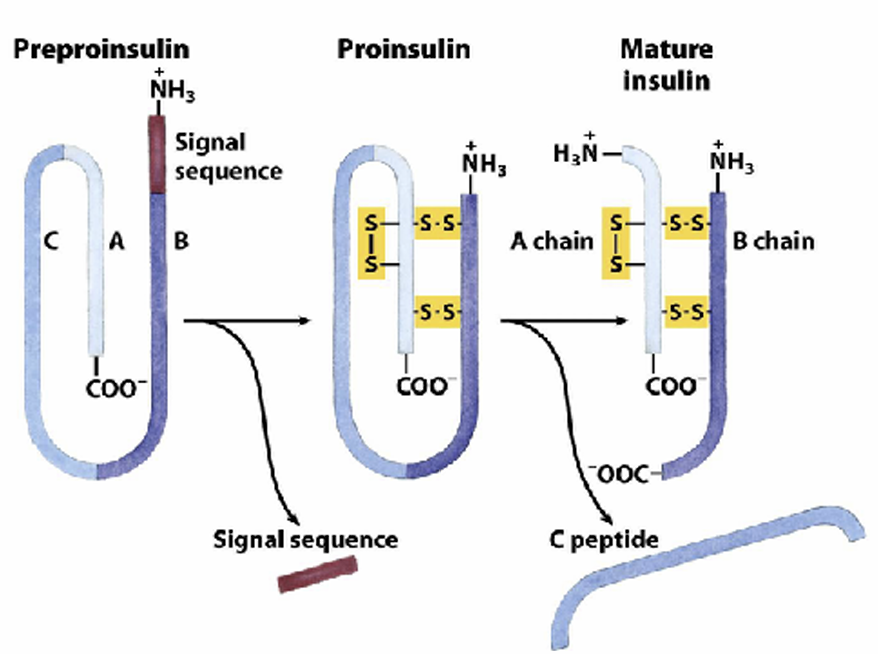
\includegraphics[width=0.5\linewidth]{insulinProduction.png}
    \caption{insulin processing}
    \label{fig:enter-label}
\end{figure}
Preporinsulin has 3 chains A, B and C and an ER localization signal. chains\textbf{ A and B are linked by disulfide bonds}, while \textbf{chain C is cleaved off} this is done by \textbf{prohormone convertases} (\gls{pc1pc2}), as well as the 
\textbf{exoprotease \gls{cpe}}
\paragraph{insulin response pathway in other cells}
(the professor didn't talk much about this but I'll add it in just in case)
\begin{figure}[H]
    \centering
    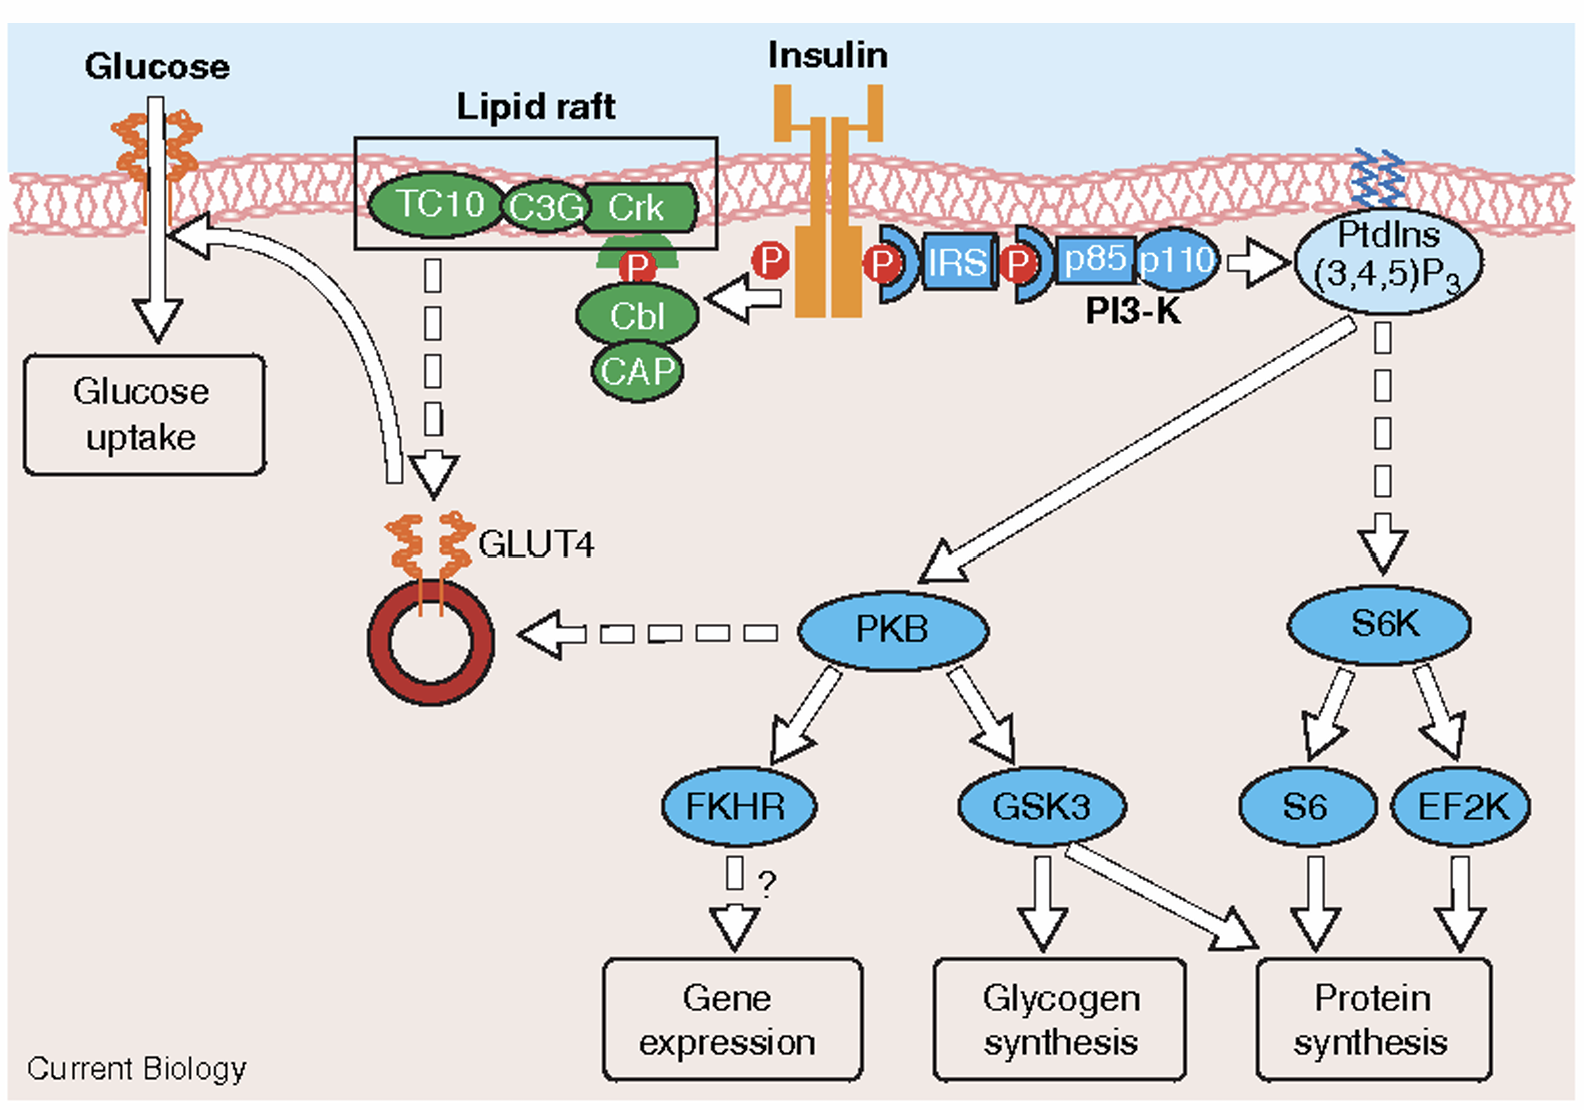
\includegraphics[width=0.7\linewidth]{insulinPathway.png}
    \caption{insulin pathway}
    \label{fig:enter-label}
\end{figure}
Insulin pathway is a classical example of\textbf{ RTK receptor signaliling}
\paragraph{effects of insulin table}
\begin{figure}[H]
    \centering
    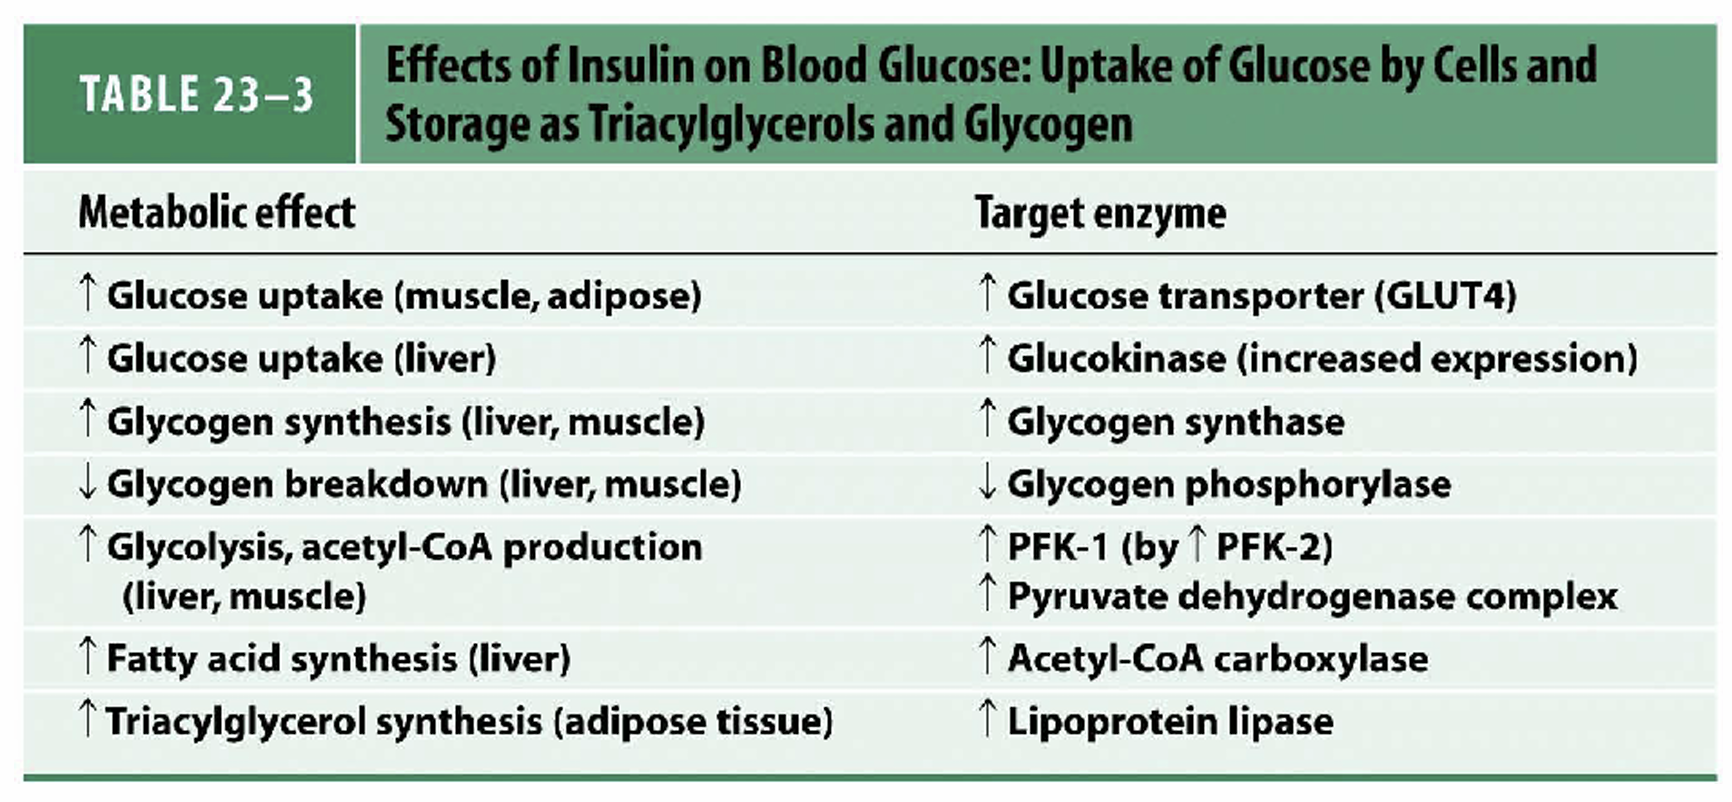
\includegraphics[width=\linewidth]{insulinTable.png}
    \caption{table of insulin effects}
    \label{fig:enter-label}
\end{figure}

\subsubsection{alpha cells}
\paragraph{release mechanism}
Like insulin $\alpha$-cells sense the glucose concentration via the concentration of produced ATP.
\begin{enumerate}
    \item high ATP concentration inhibits ATP-gated K+ channels
    \item This will cause the membrane to depolarize, which will\textbf{ activate a ca2+ voltage gated channels. }
    \item the \textbf{influx of calcium} into the cell from the outside aswell as the ER, will cause the fusion of insulin granues to fuse with the membrane and be released via the \textbf{\gls{snarecomplex}} \textbf{However in $\alpha$-cells this happens at much lower glucose concentrations. and if the ATP concetration too much deplolarization will cause the closure of the ca2+ voltage gated channels}
\end{enumerate}
\paragraph{glucagon response pathway in other cells}
\begin{figure}[H]
    \centering
    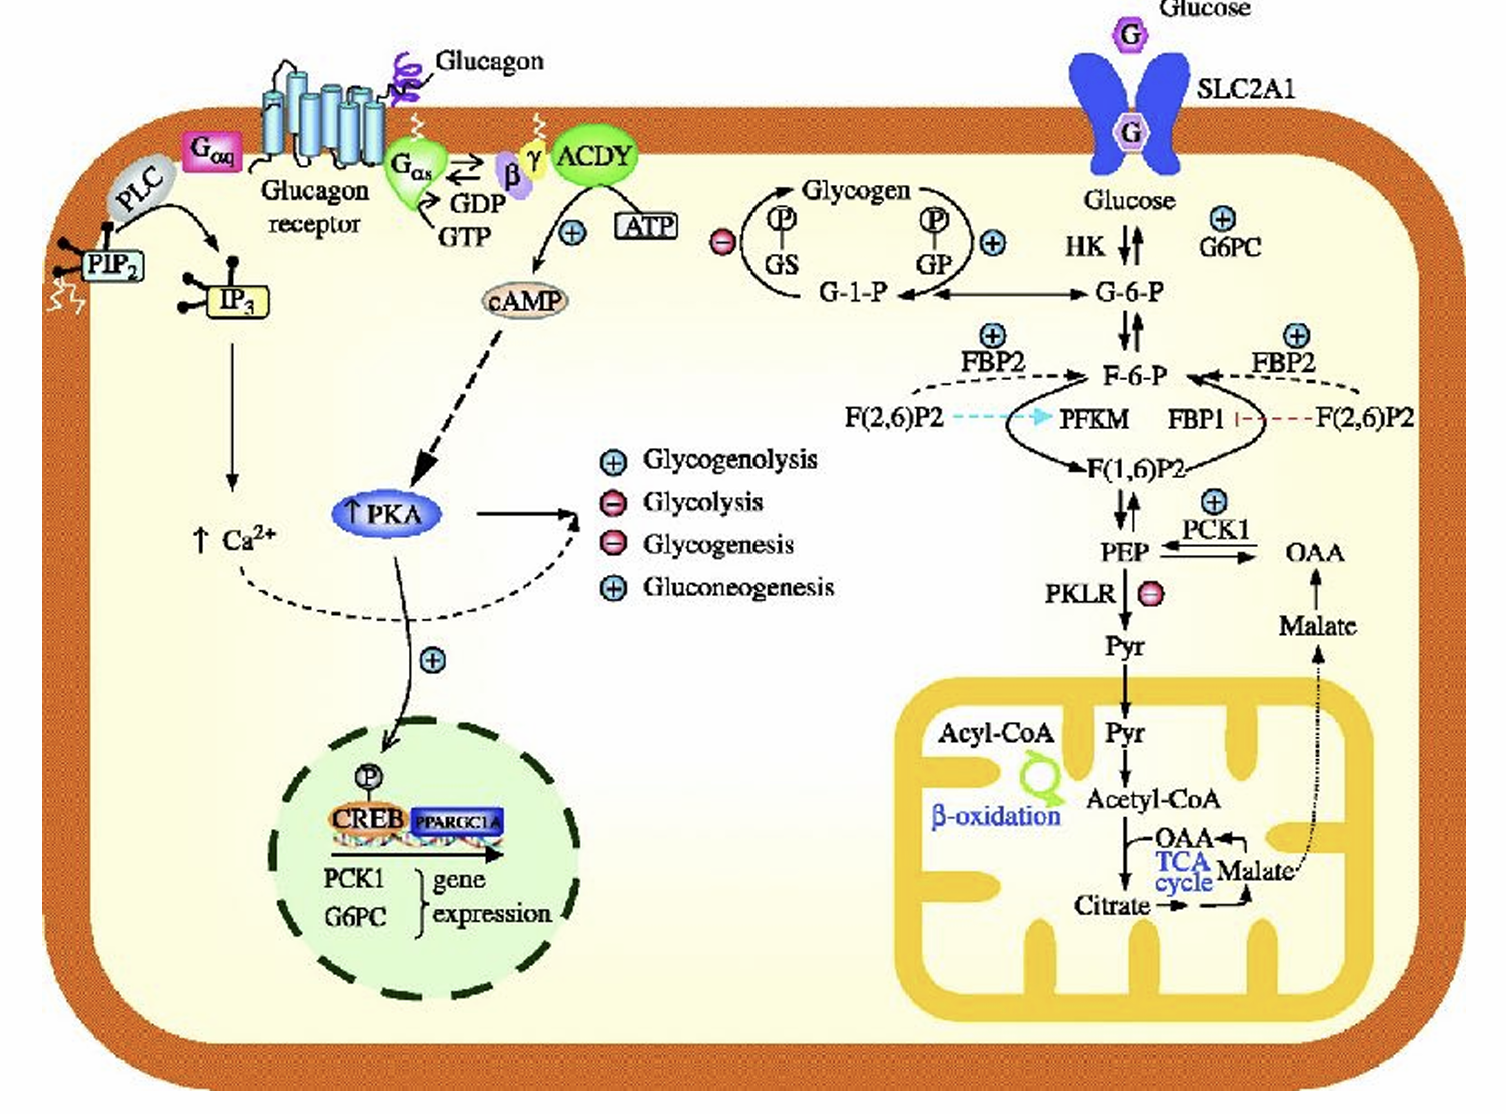
\includegraphics[width=0.5\linewidth]{GlucagonPathway.png}
    \caption{Glucagon pathway}
    \label{fig:enter-label}
\end{figure}
Glucagon pathway works over a \textbf{GPCR}

\paragraph{effect of glucagon}
\begin{figure}[H]
    \centering
    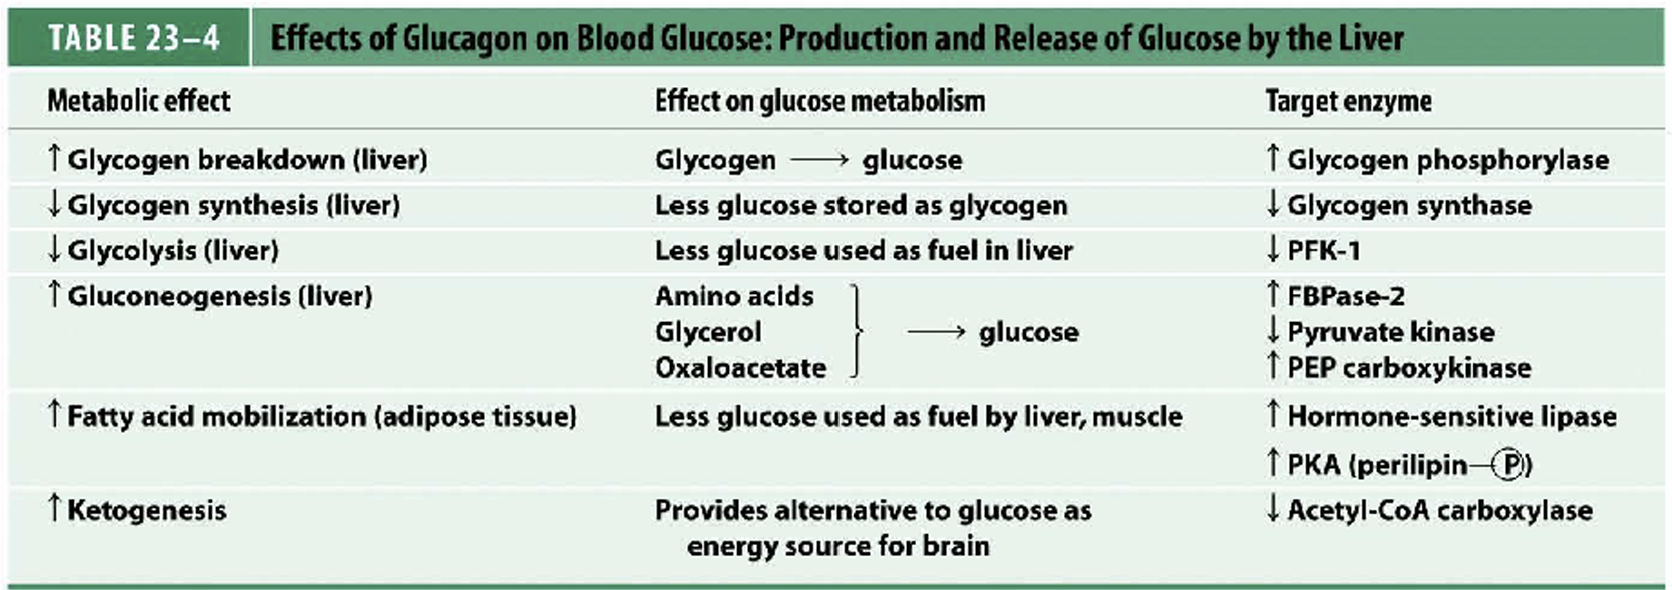
\includegraphics[width=1\linewidth]{glucagonTable.png}
    \caption{table of glucagon effects}
    \label{fig:enter-label}
\end{figure}

\subsubsection{diabetes}
\begin{figure}[H]
    \centering
    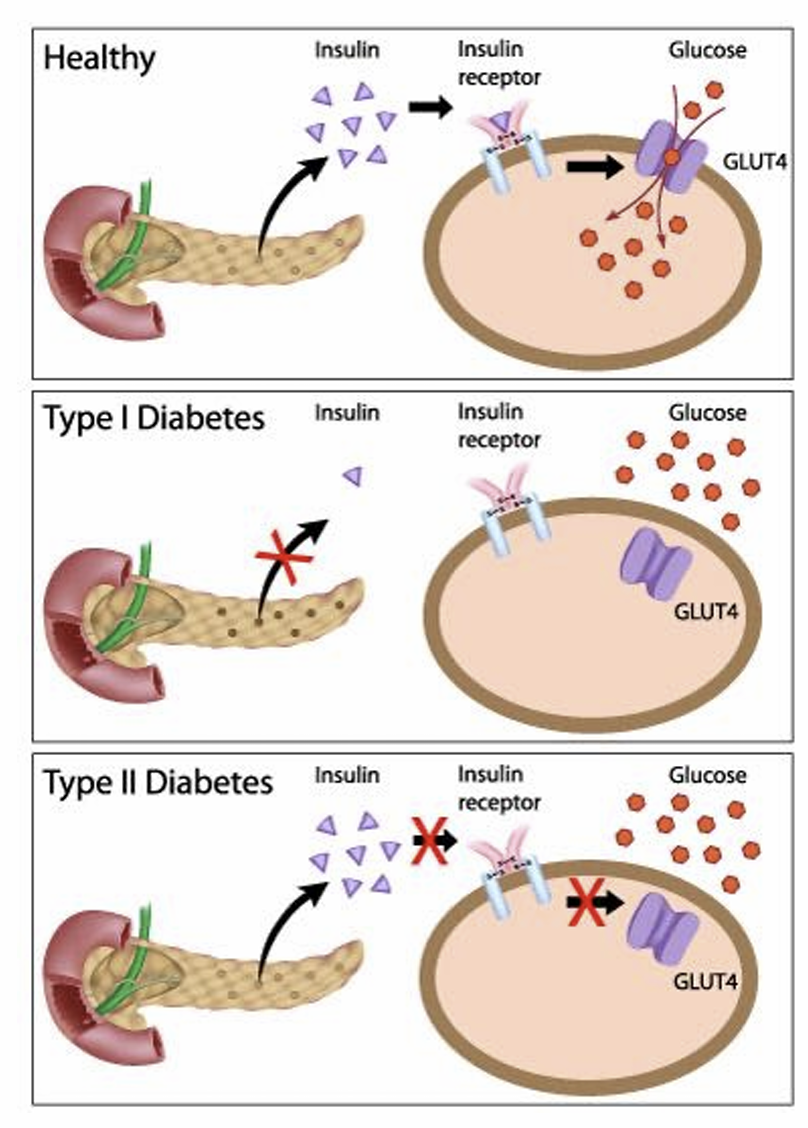
\includegraphics[width=0.5\linewidth]{diabetes.png}
    \caption{diabetes types}
    \label{fig:enter-label}
\end{figure}
There are two types of diabetes:
\begin{itemize}
    \item \textbf{Type1 diabetes:} This is an autoimmune disease where the insulin producing $\beta$-cells are destroyed. 
    \item \textbf{Type2 diabetes:} This involves a desensitization of the bodies cells to insulin due to a constatly high level of insulin. Thus loosing their ability to respond to it.
\end{itemize}




\end{document}